\chapter{Chapter 4. Results}

\section{Exploratory Model Runs}

\begin{figure}[hp!]
    \centering
    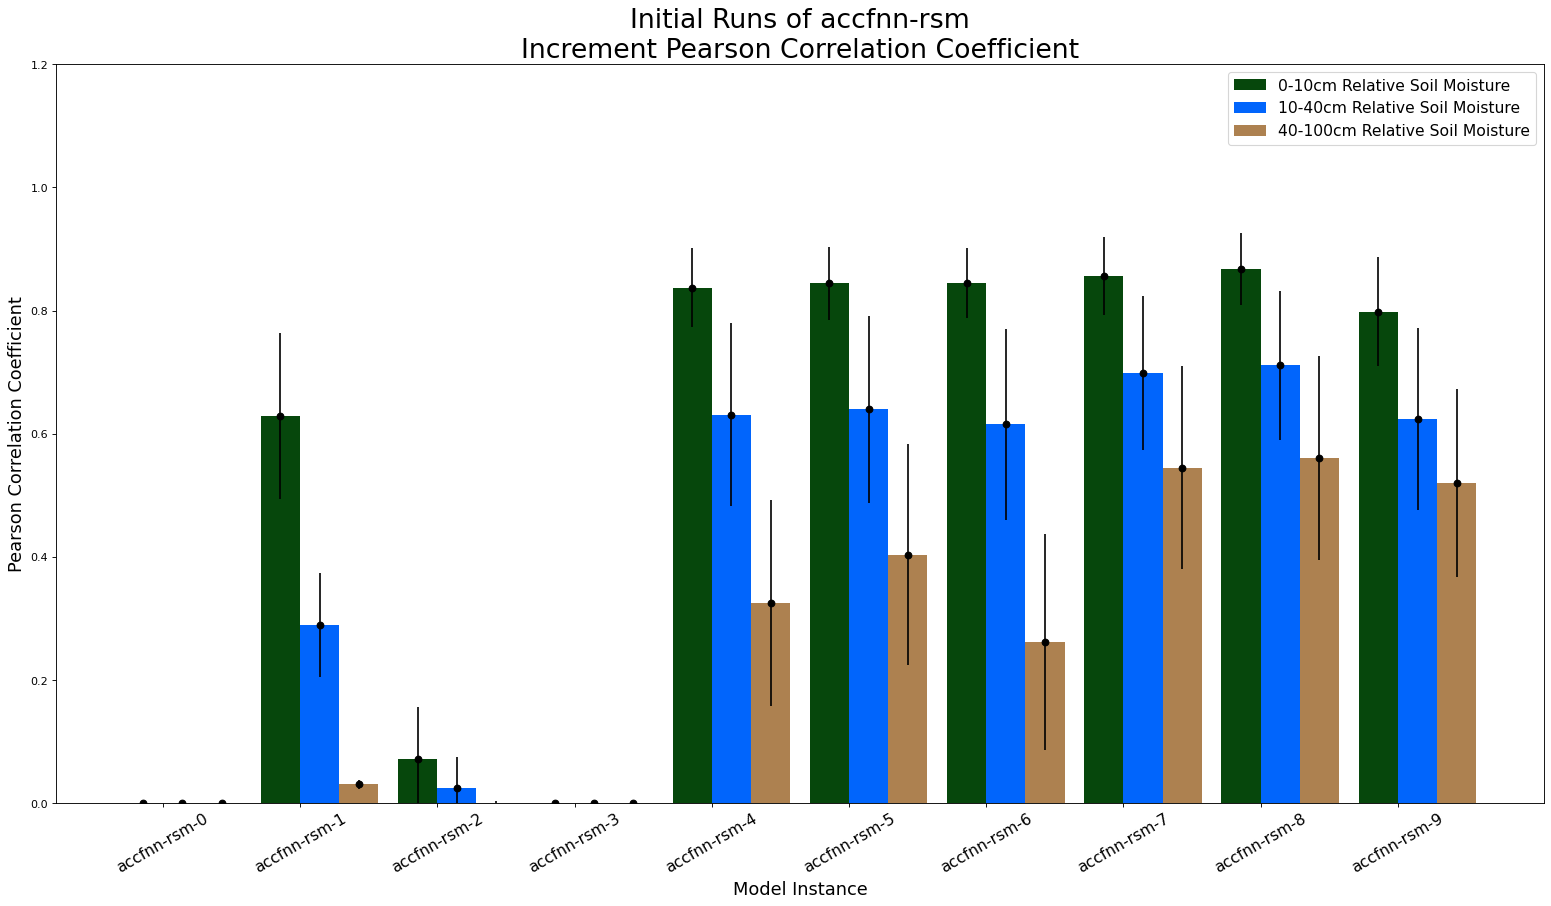
\includegraphics[width=.48\linewidth,draft=false]{figures/efficiency_initial-best/eval_test_efficiency_initial-accfnn-rsm_cc_res.png}
    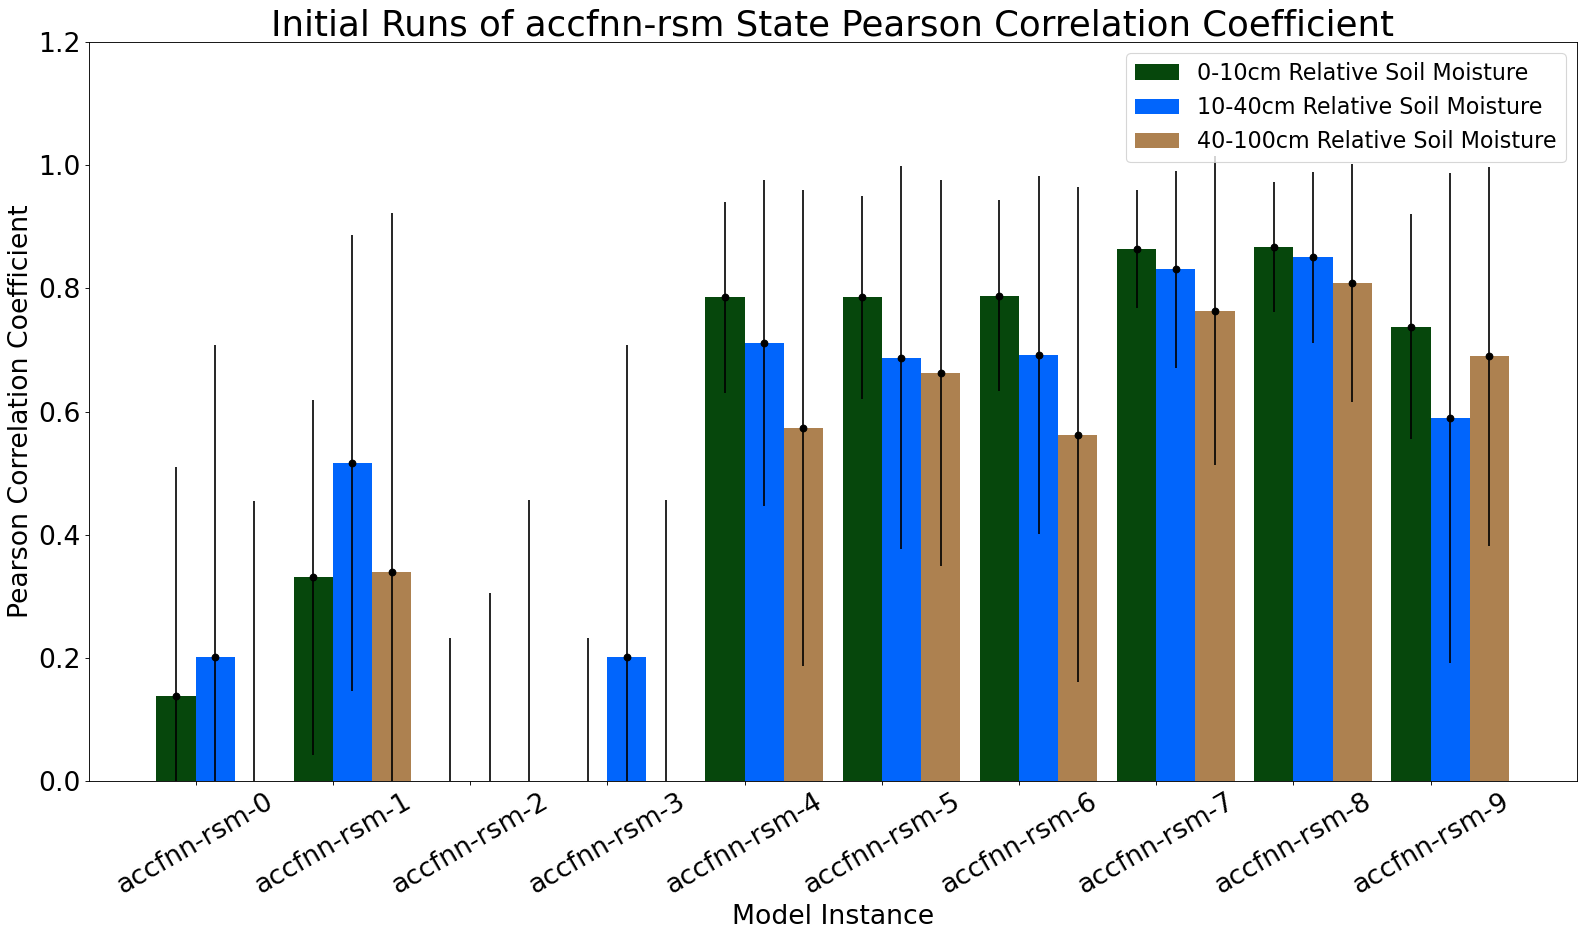
\includegraphics[width=.48\linewidth,draft=false]{figures/efficiency_initial-best/eval_test_efficiency_initial-accfnn-rsm_cc_state.png}

    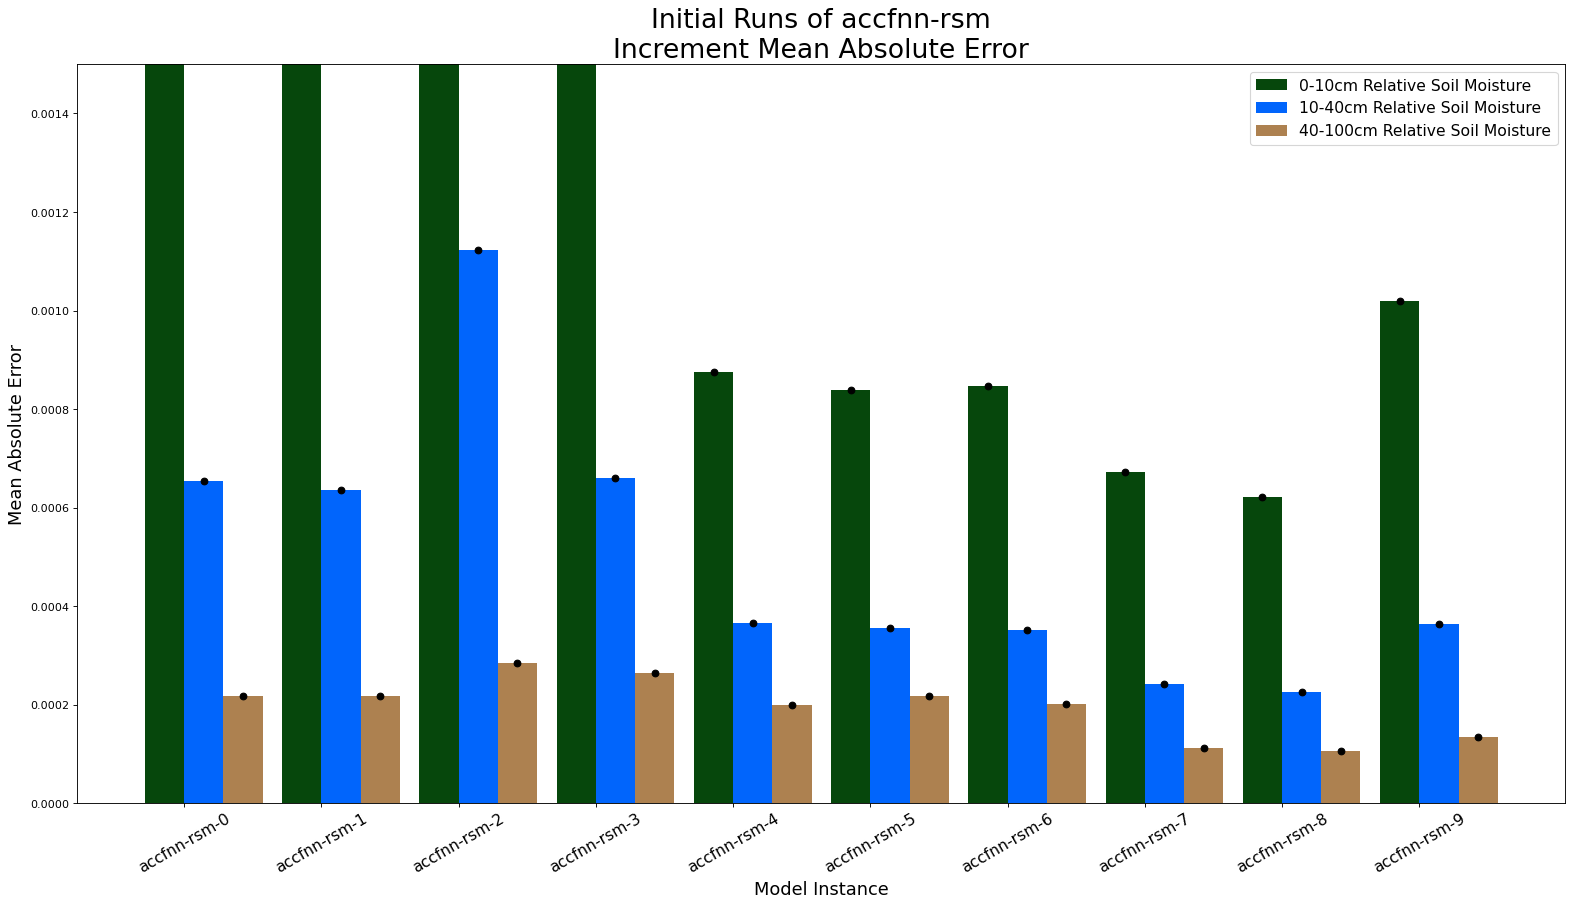
\includegraphics[width=.48\linewidth,draft=false]{figures/efficiency_initial-best/eval_test_efficiency_initial-accfnn-rsm_mae_res.png}
    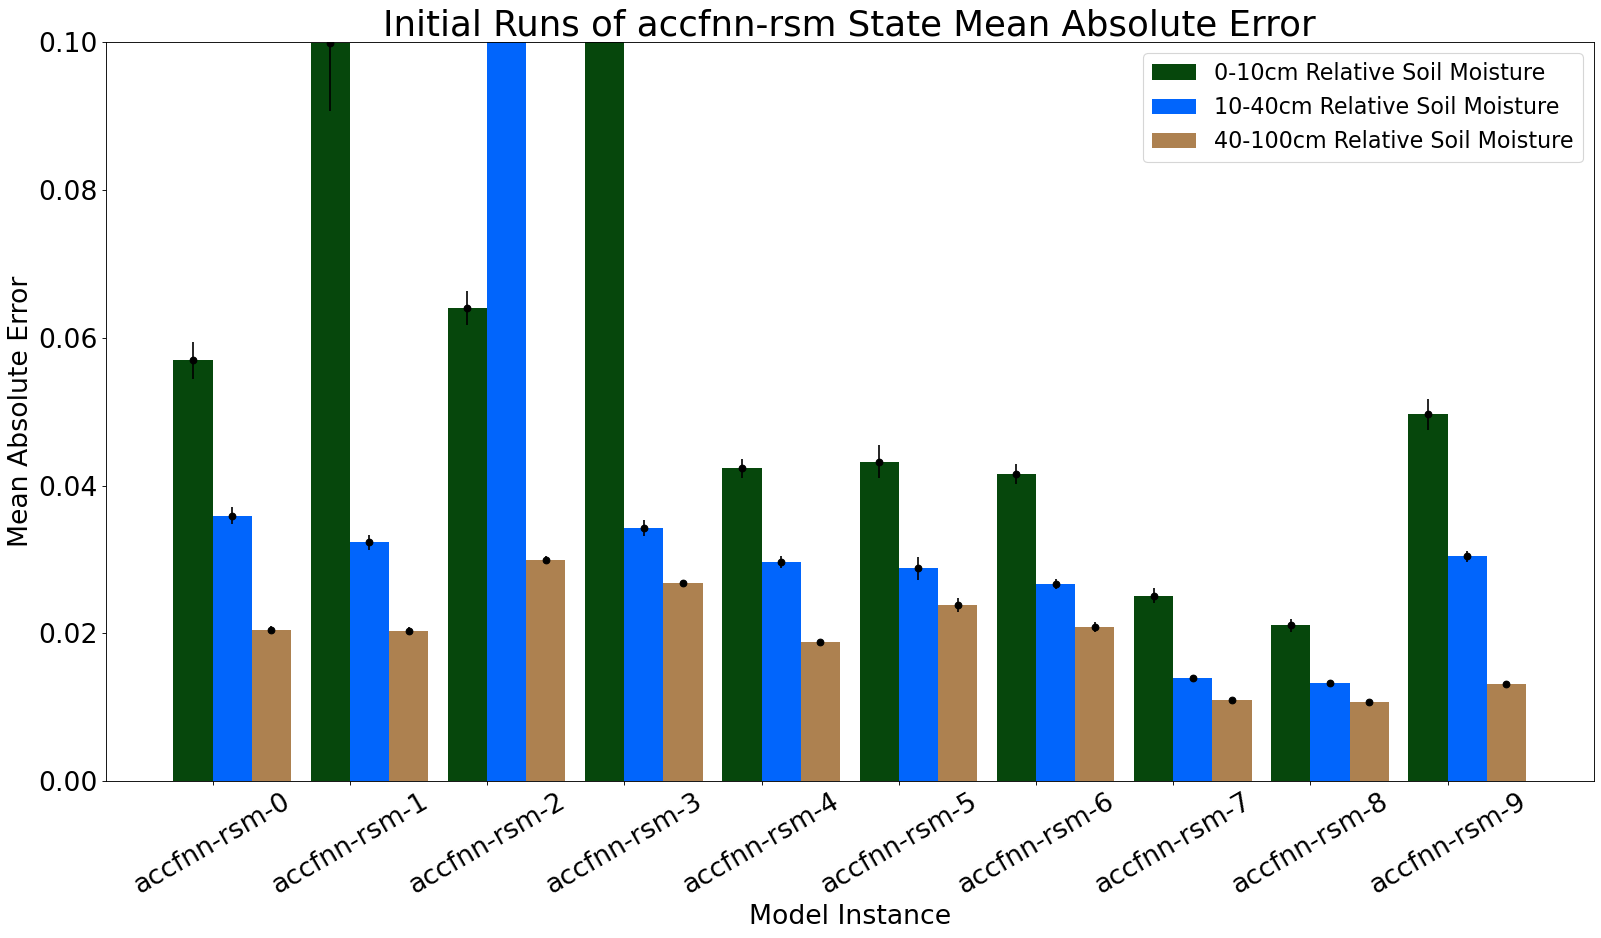
\includegraphics[width=.48\linewidth,draft=false]{figures/efficiency_initial-best/eval_test_efficiency_initial-accfnn-rsm_mae_state.png}

    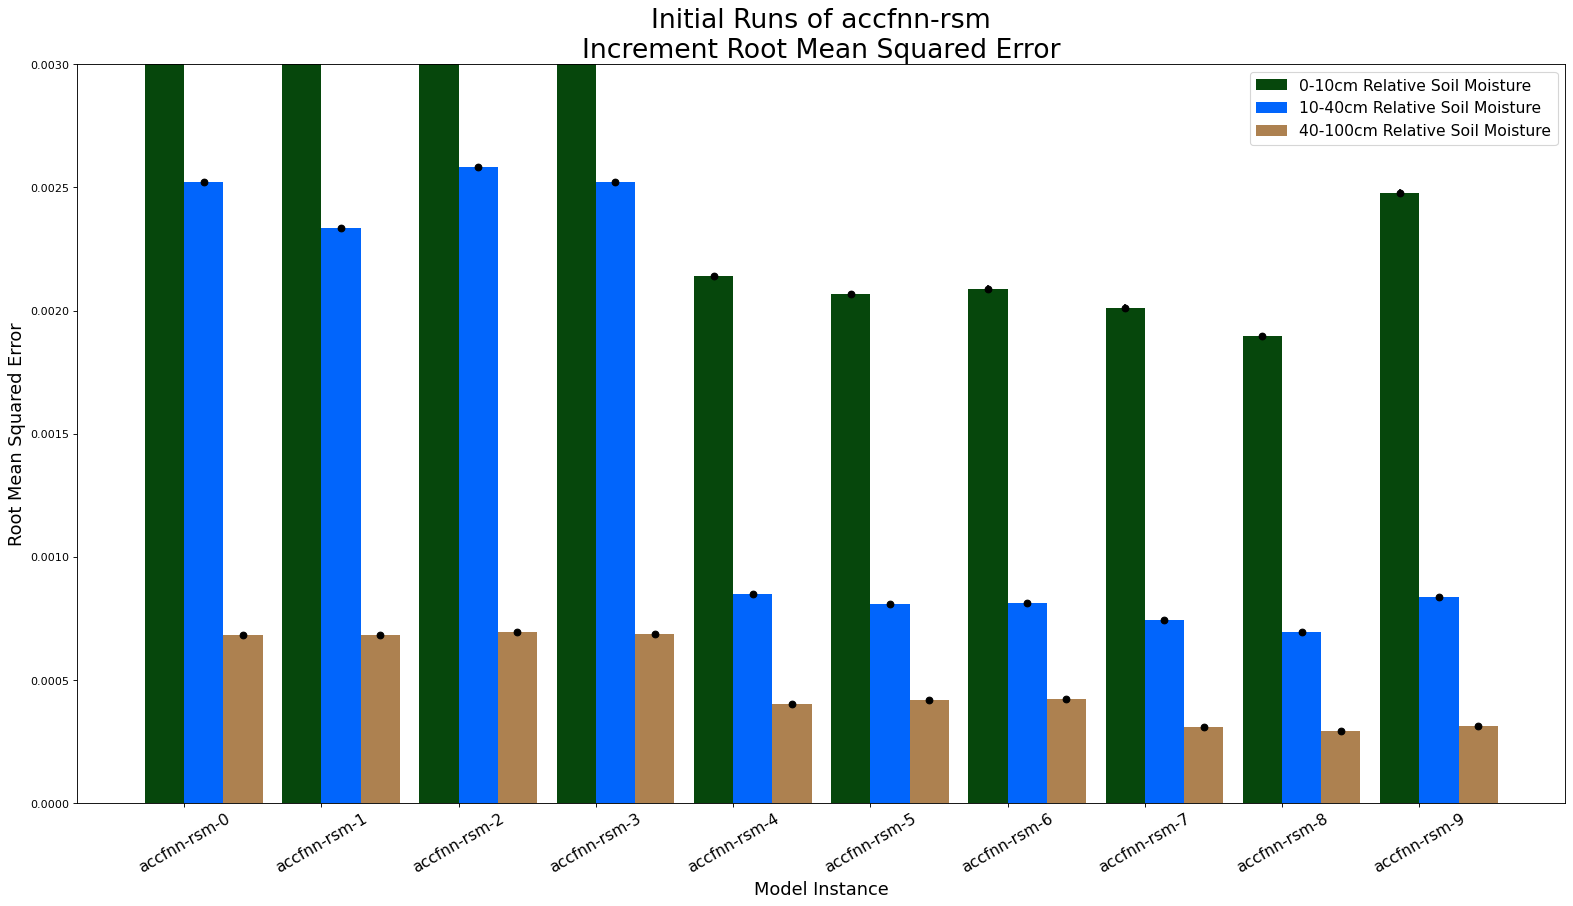
\includegraphics[width=.48\linewidth,draft=false]{figures/efficiency_initial-best/eval_test_efficiency_initial-accfnn-rsm_mse_res.png}
    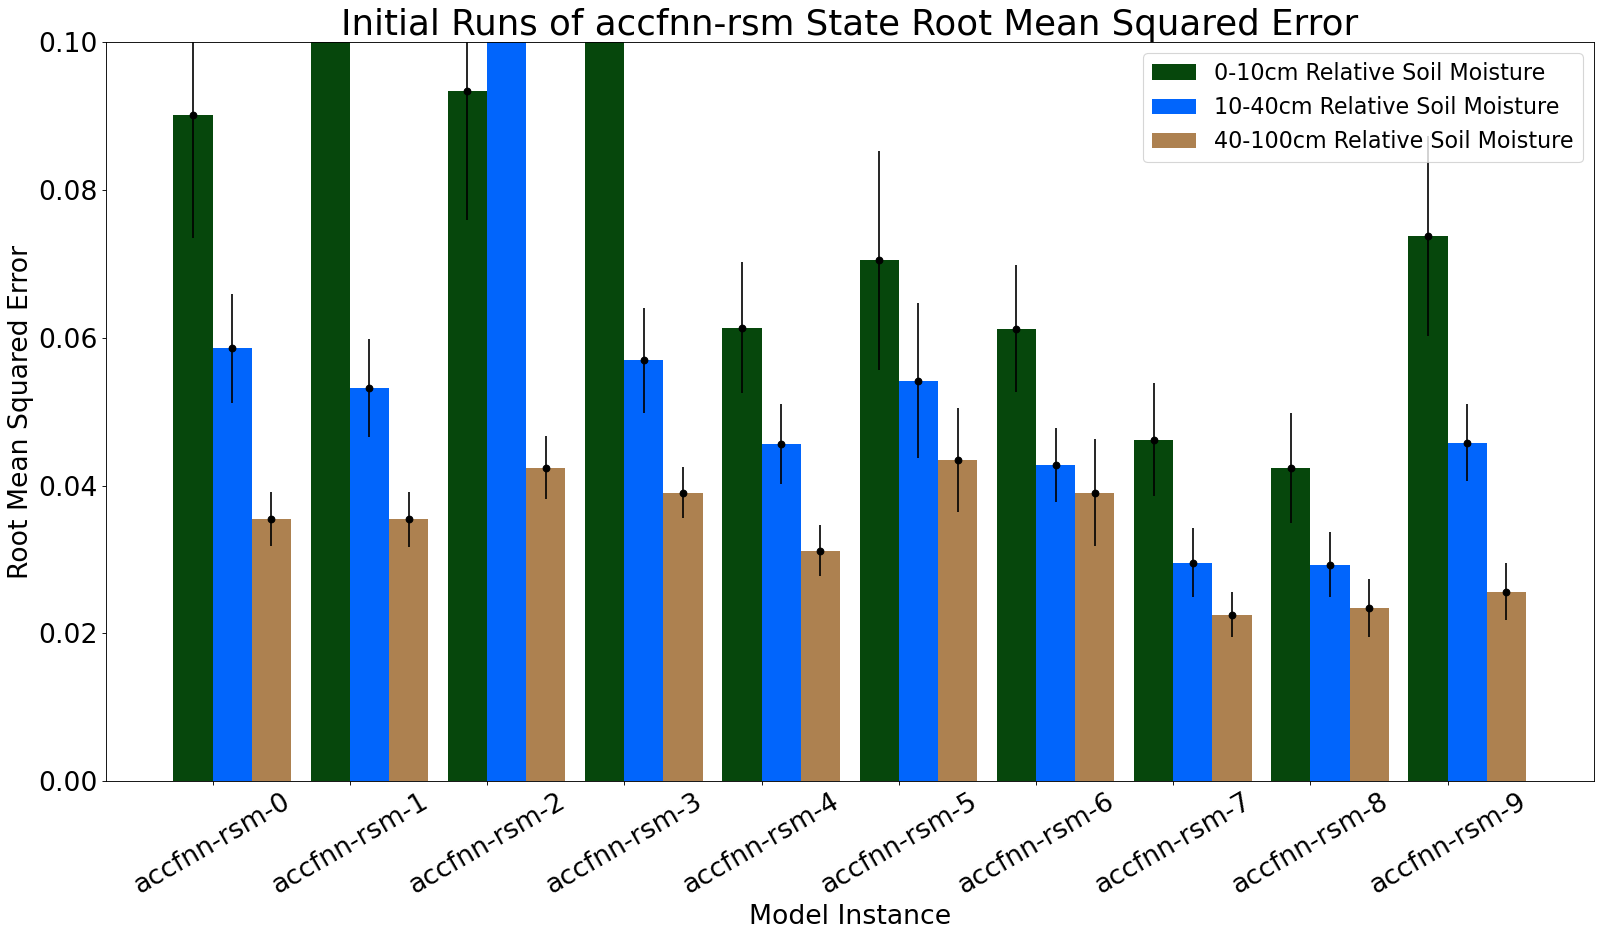
\includegraphics[width=.48\linewidth,draft=false]{figures/efficiency_initial-best/eval_test_efficiency_initial-accfnn-rsm_mse_state.png}

    \caption{Bulk metrics for initial FNN training runs}
    \label{model-init-fnn}
\end{figure}

\begin{figure}[hp!]
    \centering
    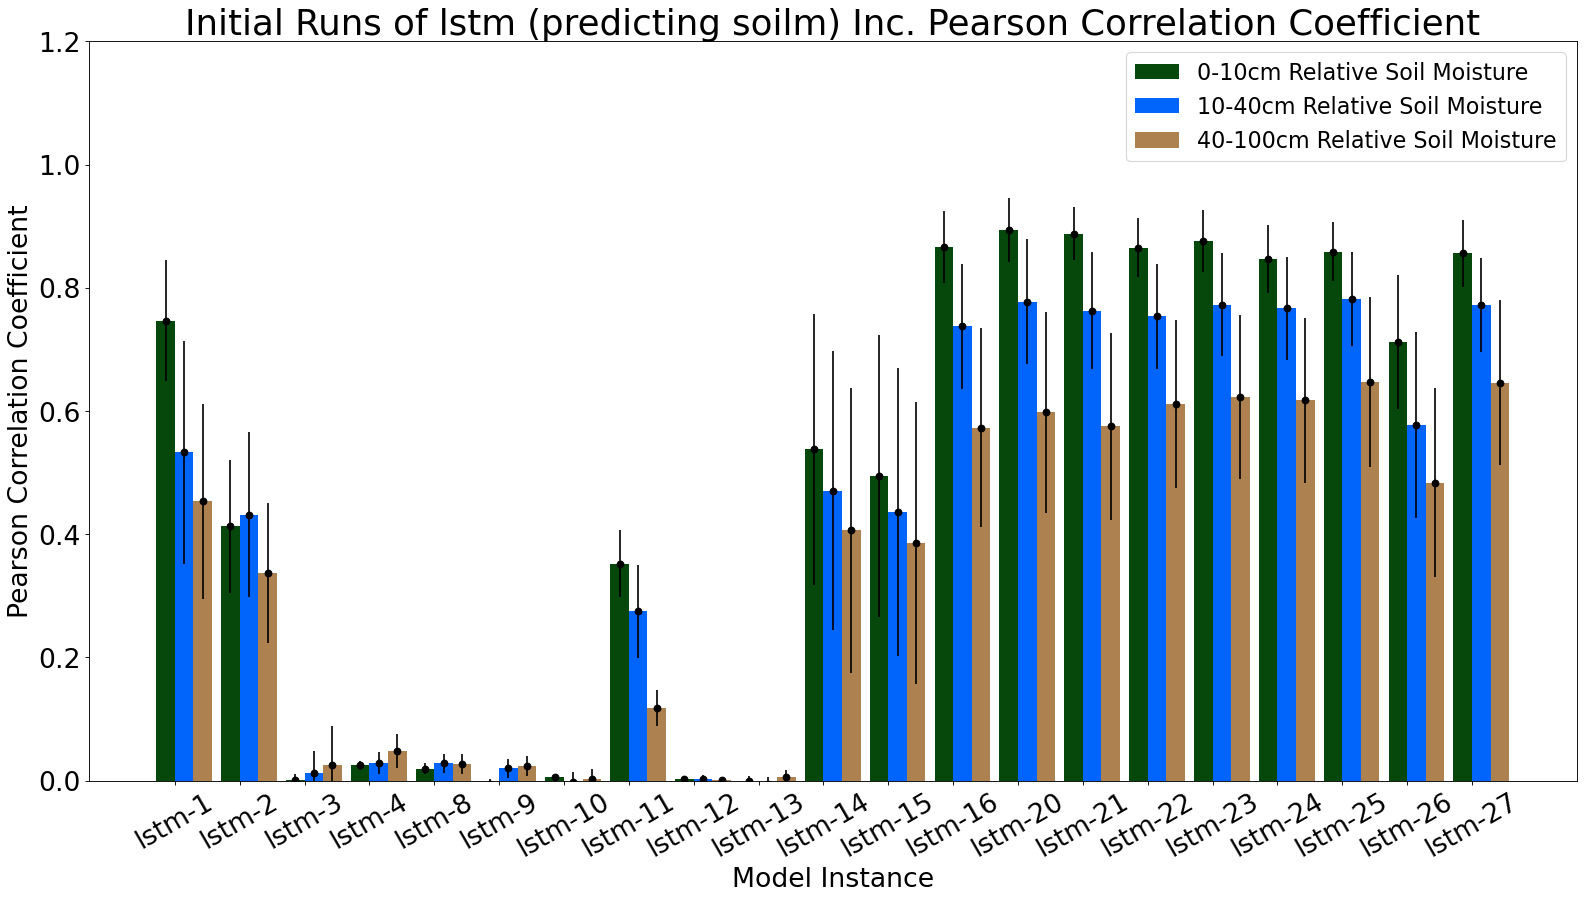
\includegraphics[width=.48\linewidth,draft=false]{figures/efficiency_initial-best/eval_test_efficiency_initial-lstm-soilm_cc_res.png}
    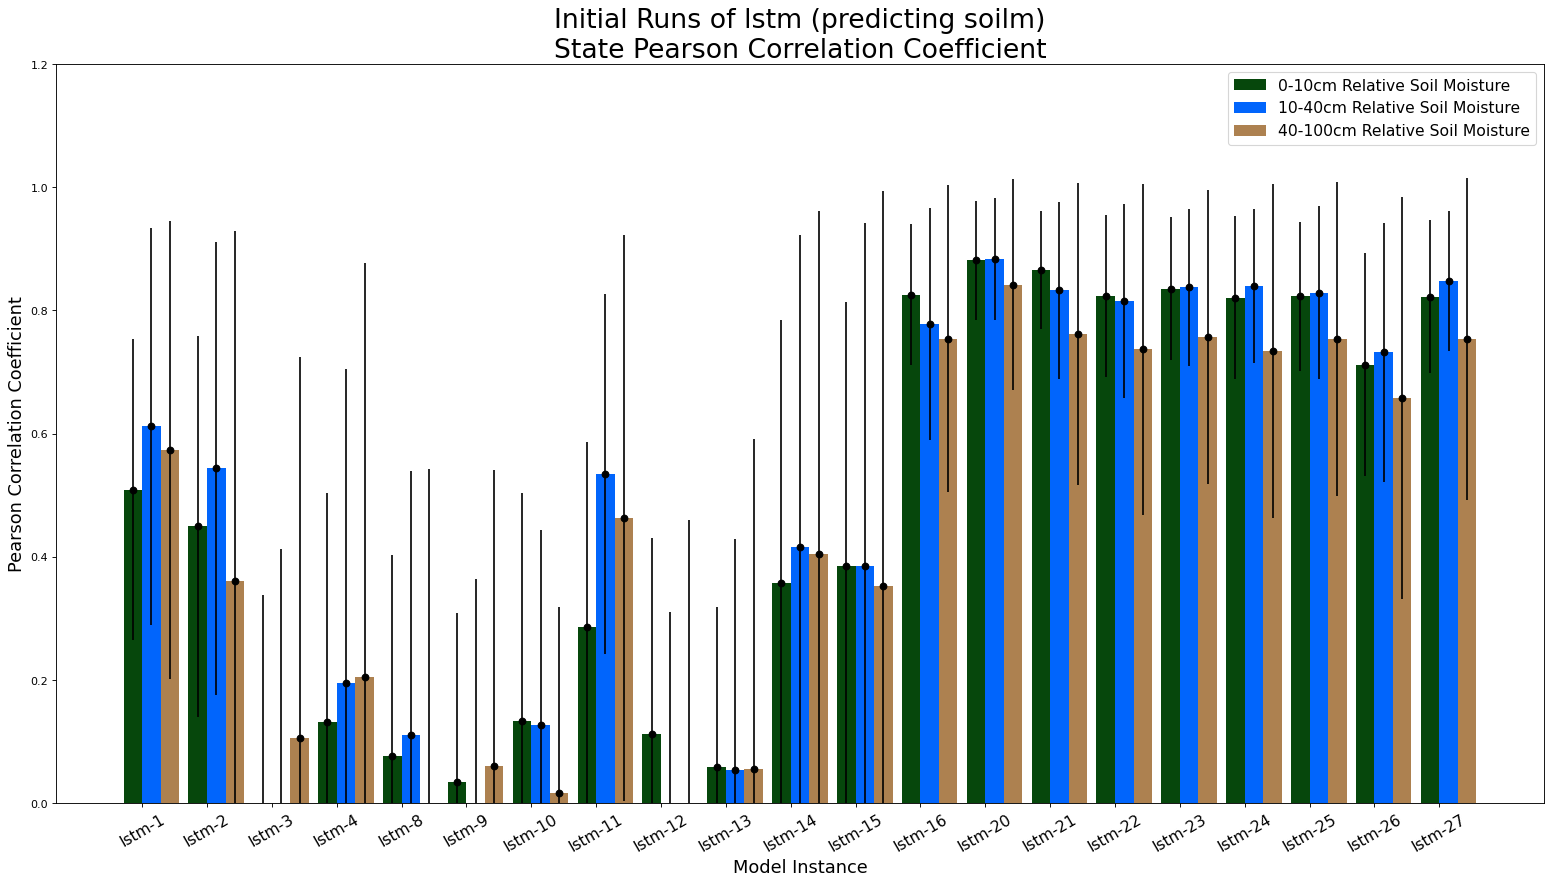
\includegraphics[width=.48\linewidth,draft=false]{figures/efficiency_initial-best/eval_test_efficiency_initial-lstm-soilm_cc_state.png}

    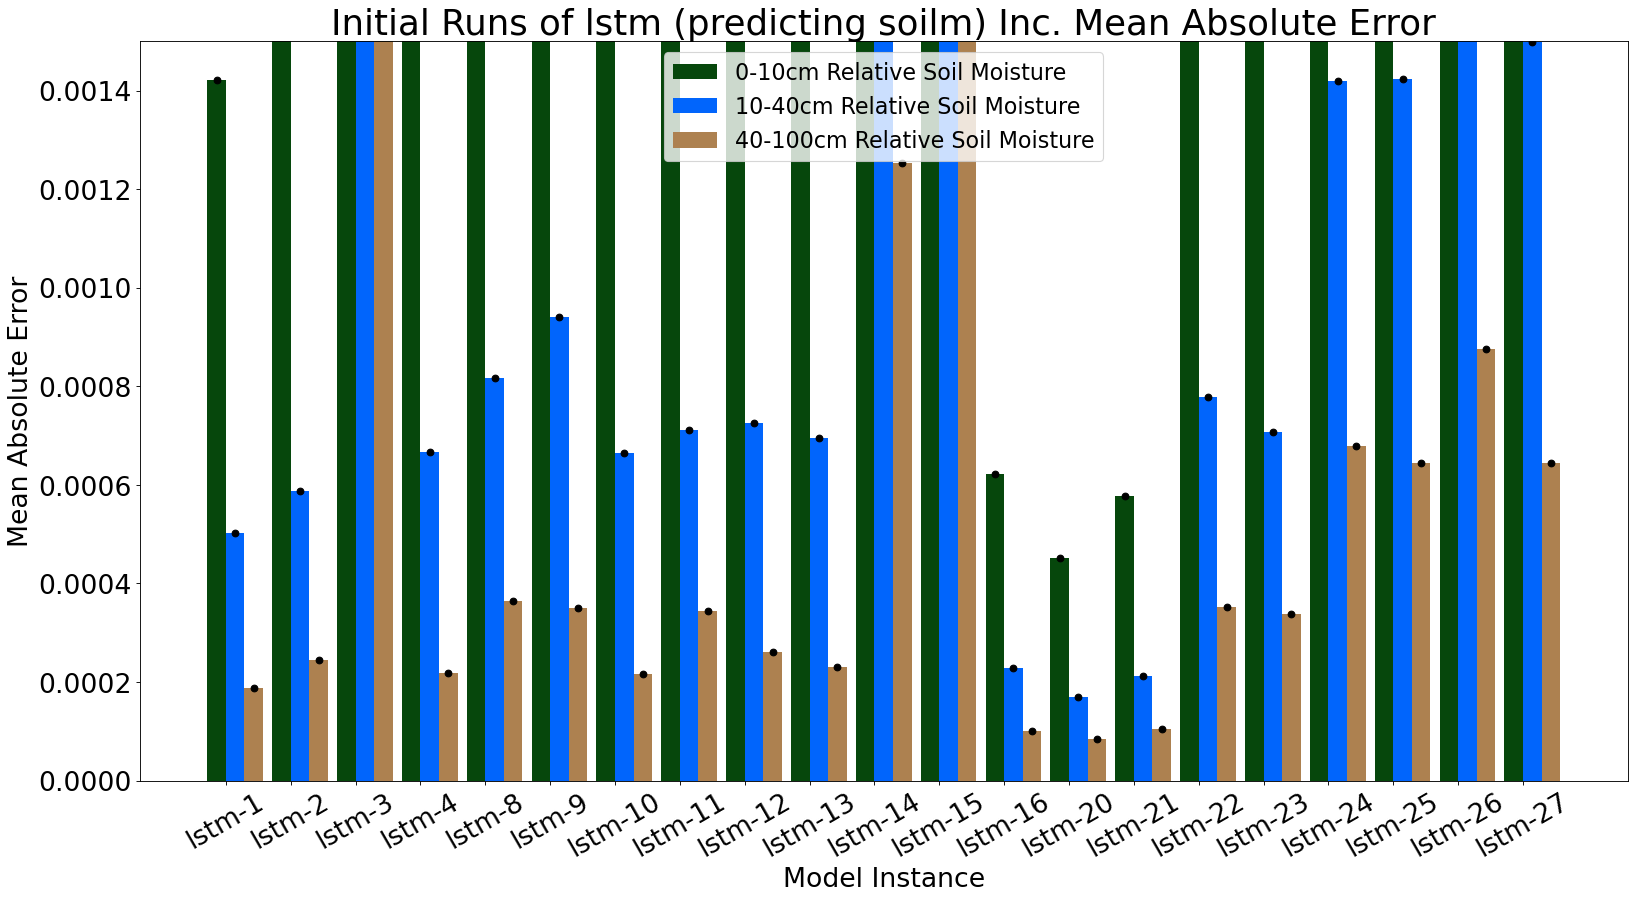
\includegraphics[width=.48\linewidth,draft=false]{figures/efficiency_initial-best/eval_test_efficiency_initial-lstm-soilm_mae_res.png}
    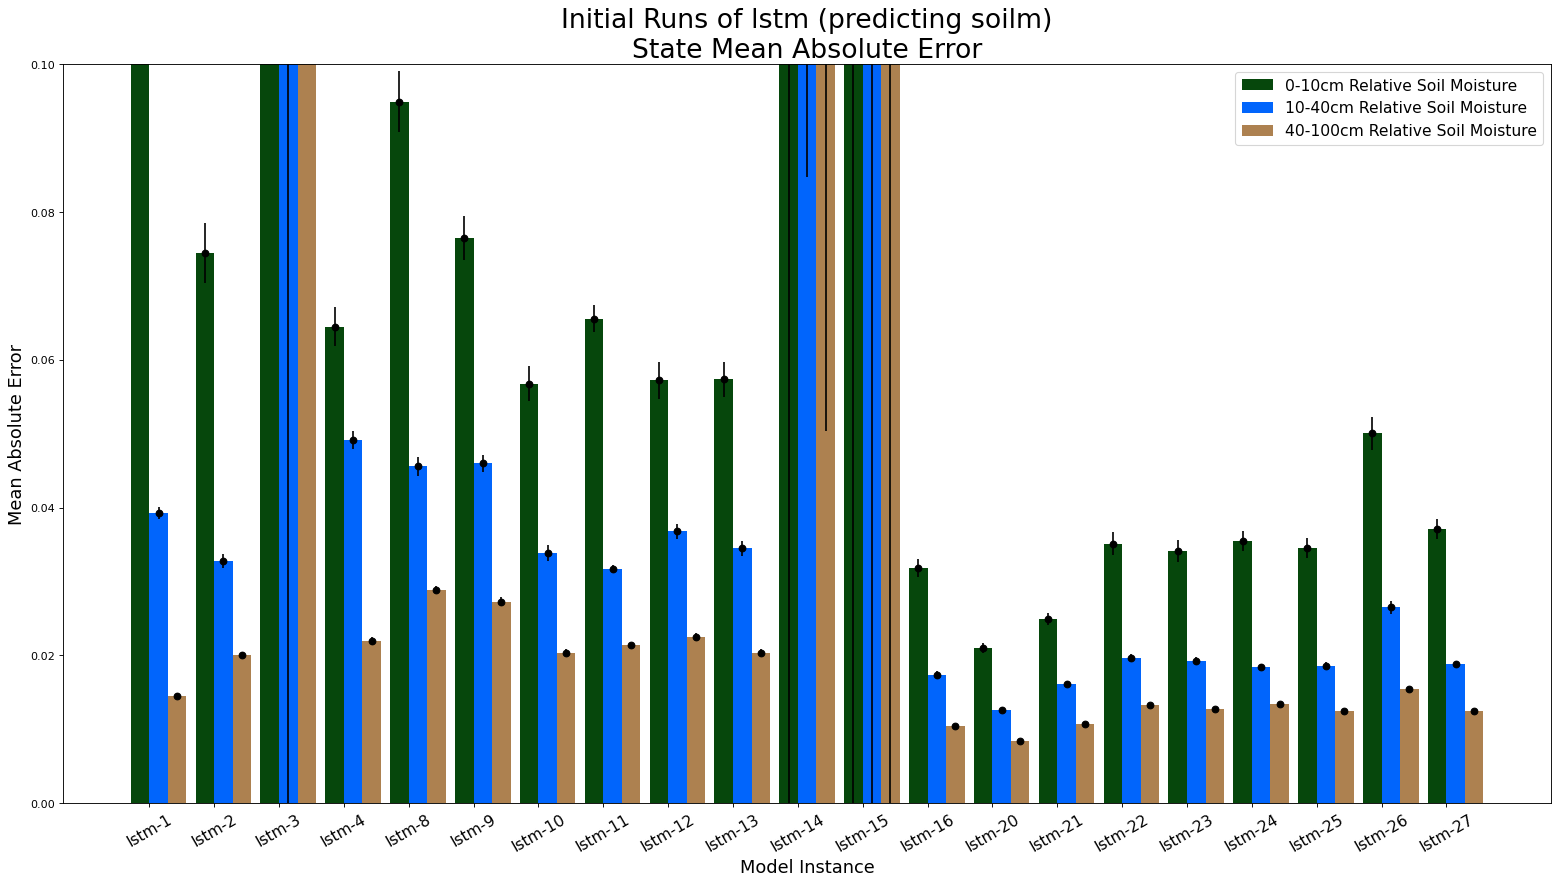
\includegraphics[width=.48\linewidth,draft=false]{figures/efficiency_initial-best/eval_test_efficiency_initial-lstm-soilm_mae_state.png}

    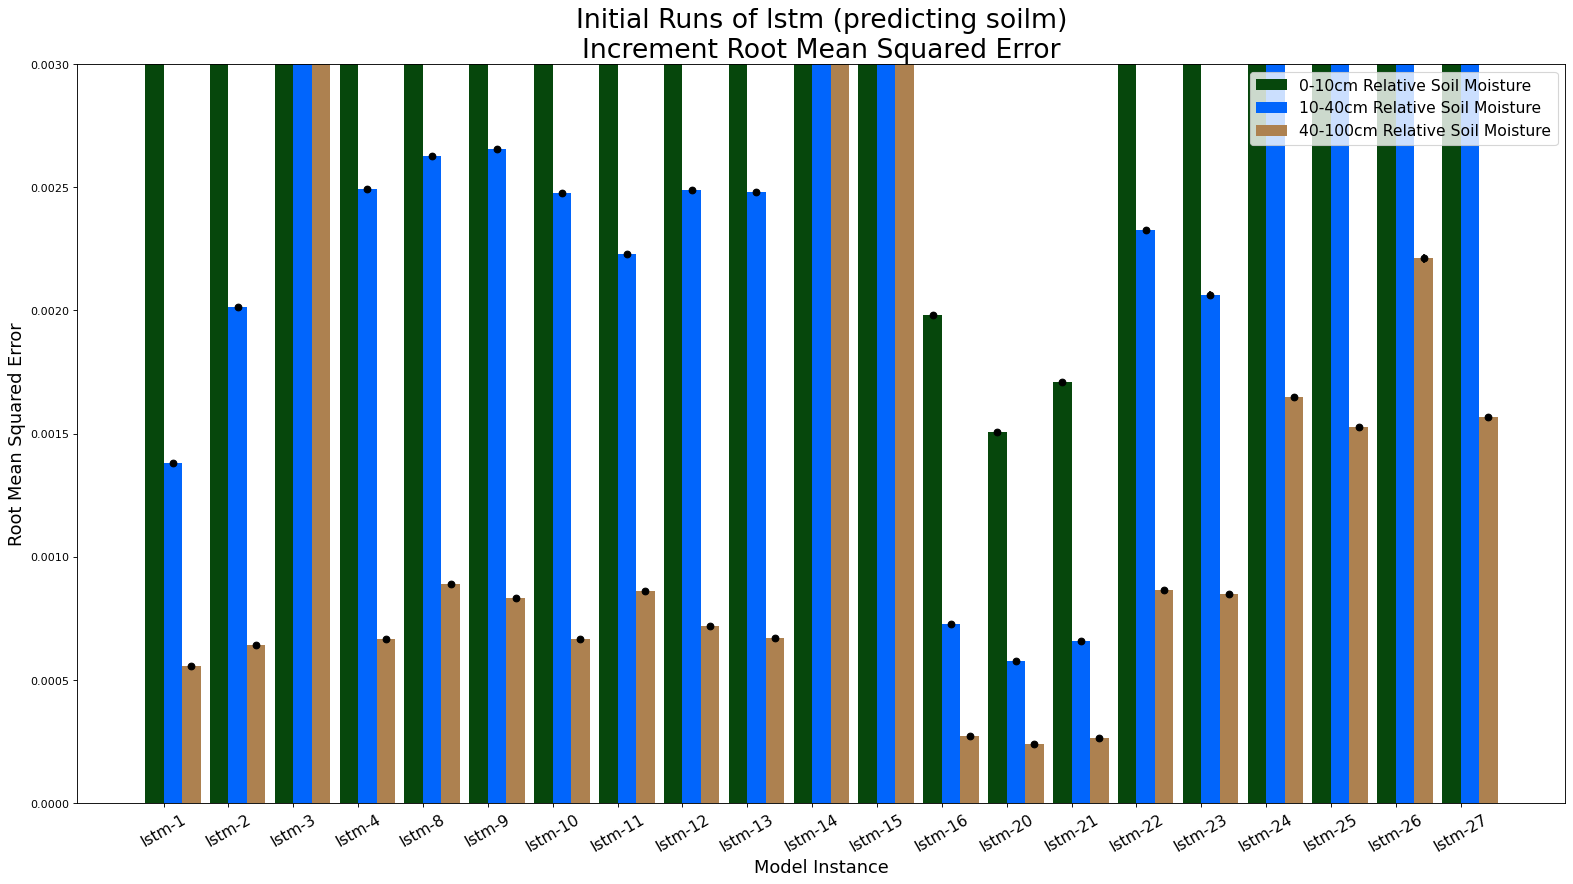
\includegraphics[width=.48\linewidth,draft=false]{figures/efficiency_initial-best/eval_test_efficiency_initial-lstm-soilm_mse_res.png}
    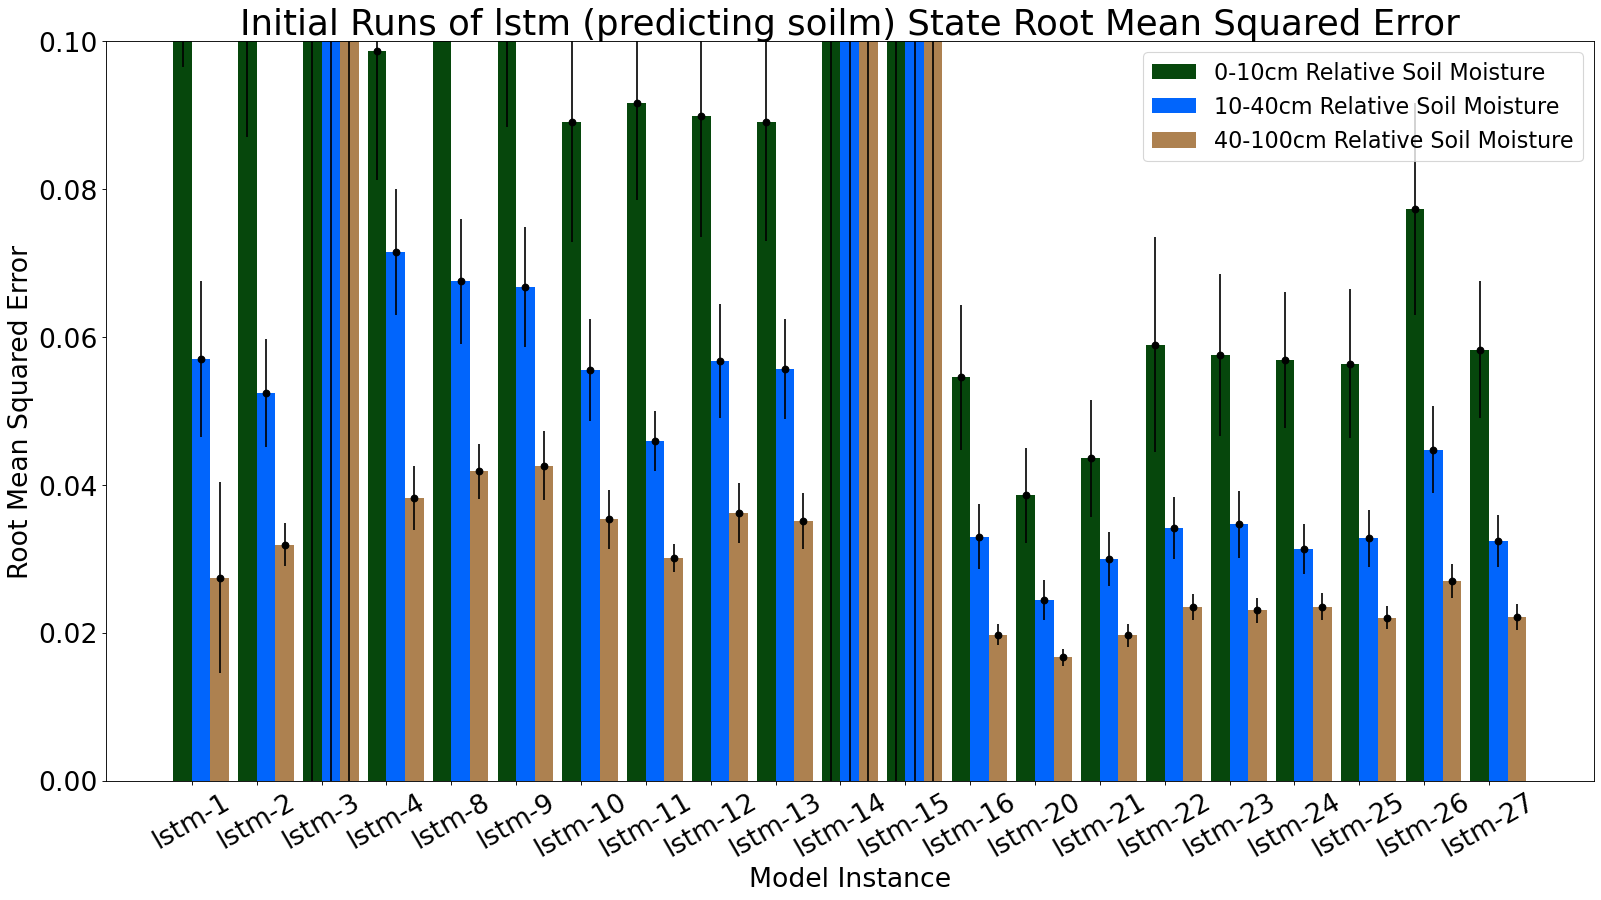
\includegraphics[width=.48\linewidth,draft=false]{figures/efficiency_initial-best/eval_test_efficiency_initial-lstm-soilm_mse_state.png}

    \caption{Bulk metrics for initial LSTM-SOILM (area density predictor) training runs}
    \label{model-init-fnn}
\end{figure}

\begin{figure}[hp!]
    \centering
    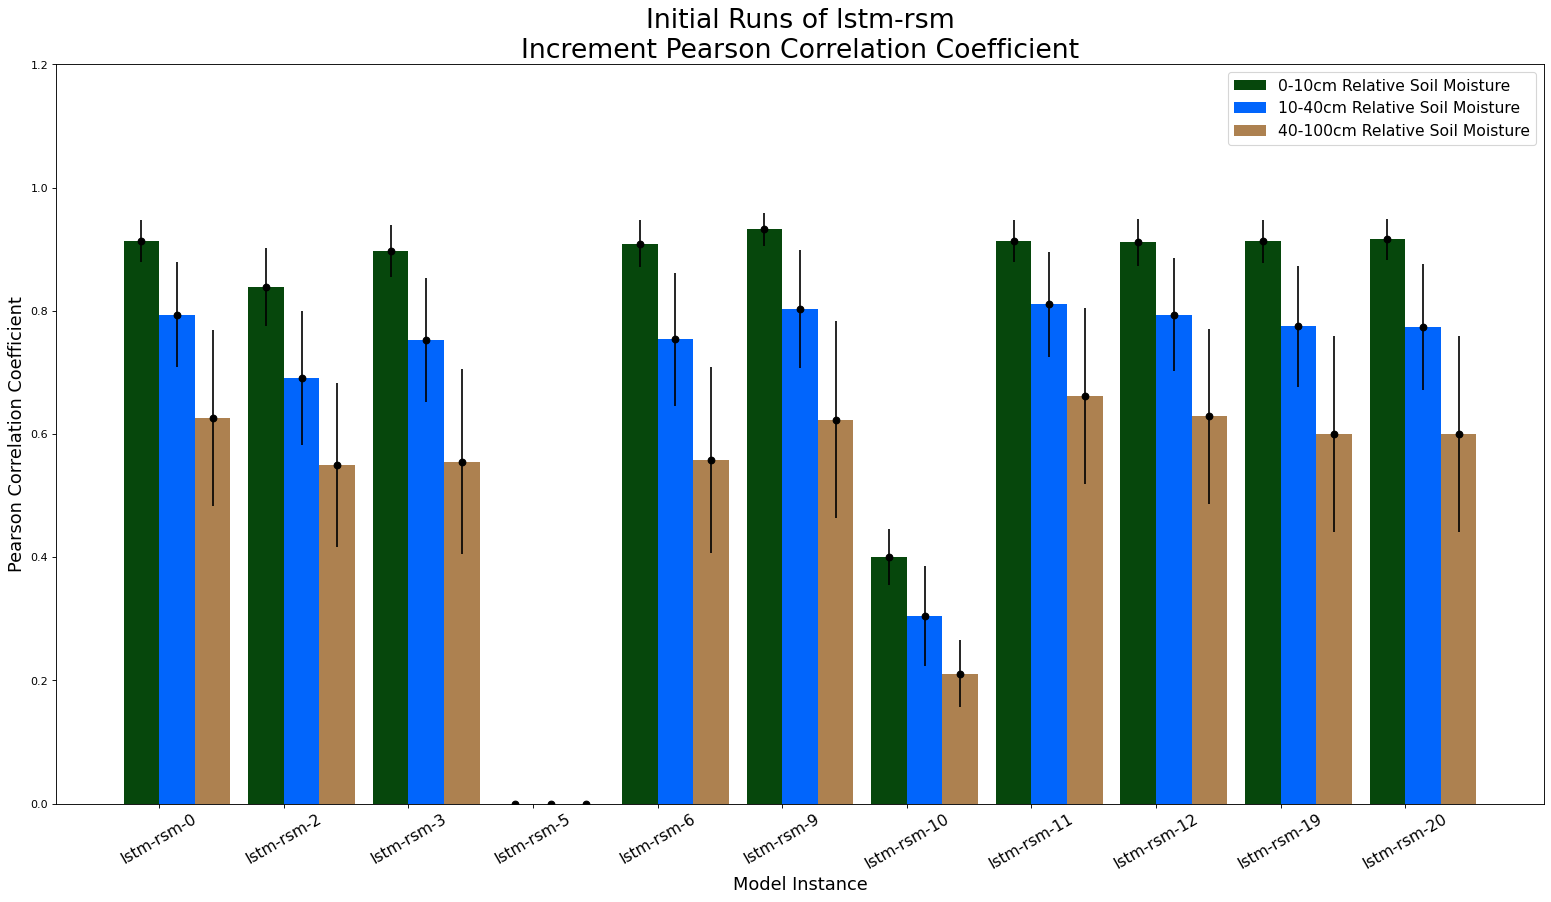
\includegraphics[width=.48\linewidth,draft=false]{figures/efficiency_initial-best/eval_test_efficiency_initial-lstm-rsm_cc_res.png}
    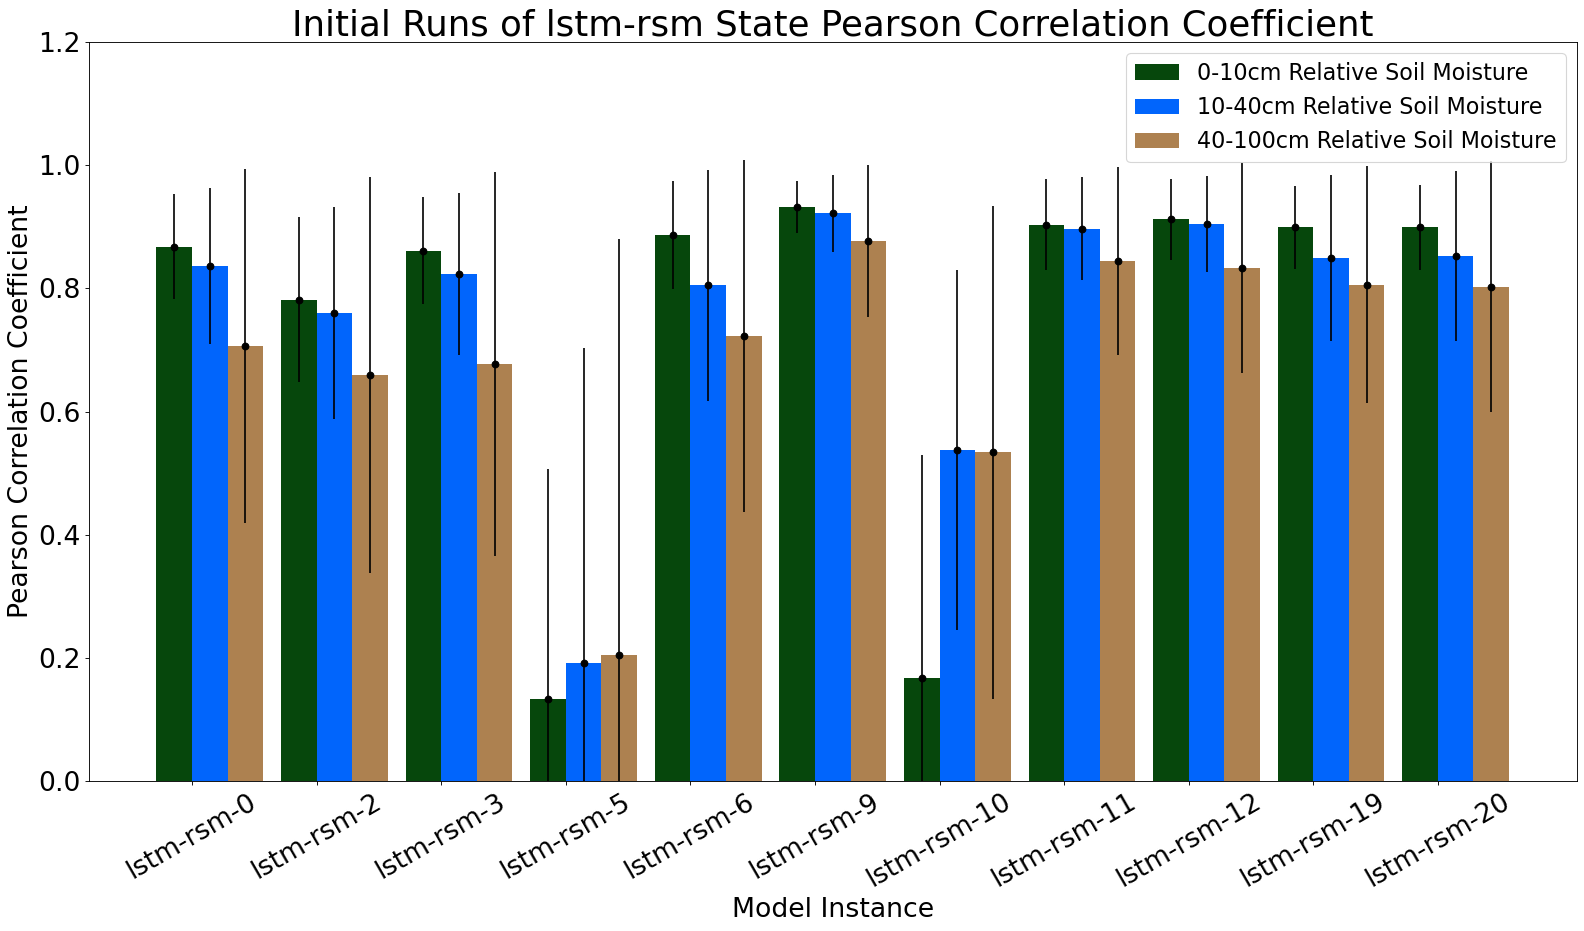
\includegraphics[width=.48\linewidth,draft=false]{figures/efficiency_initial-best/eval_test_efficiency_initial-lstm-rsm_cc_state.png}

    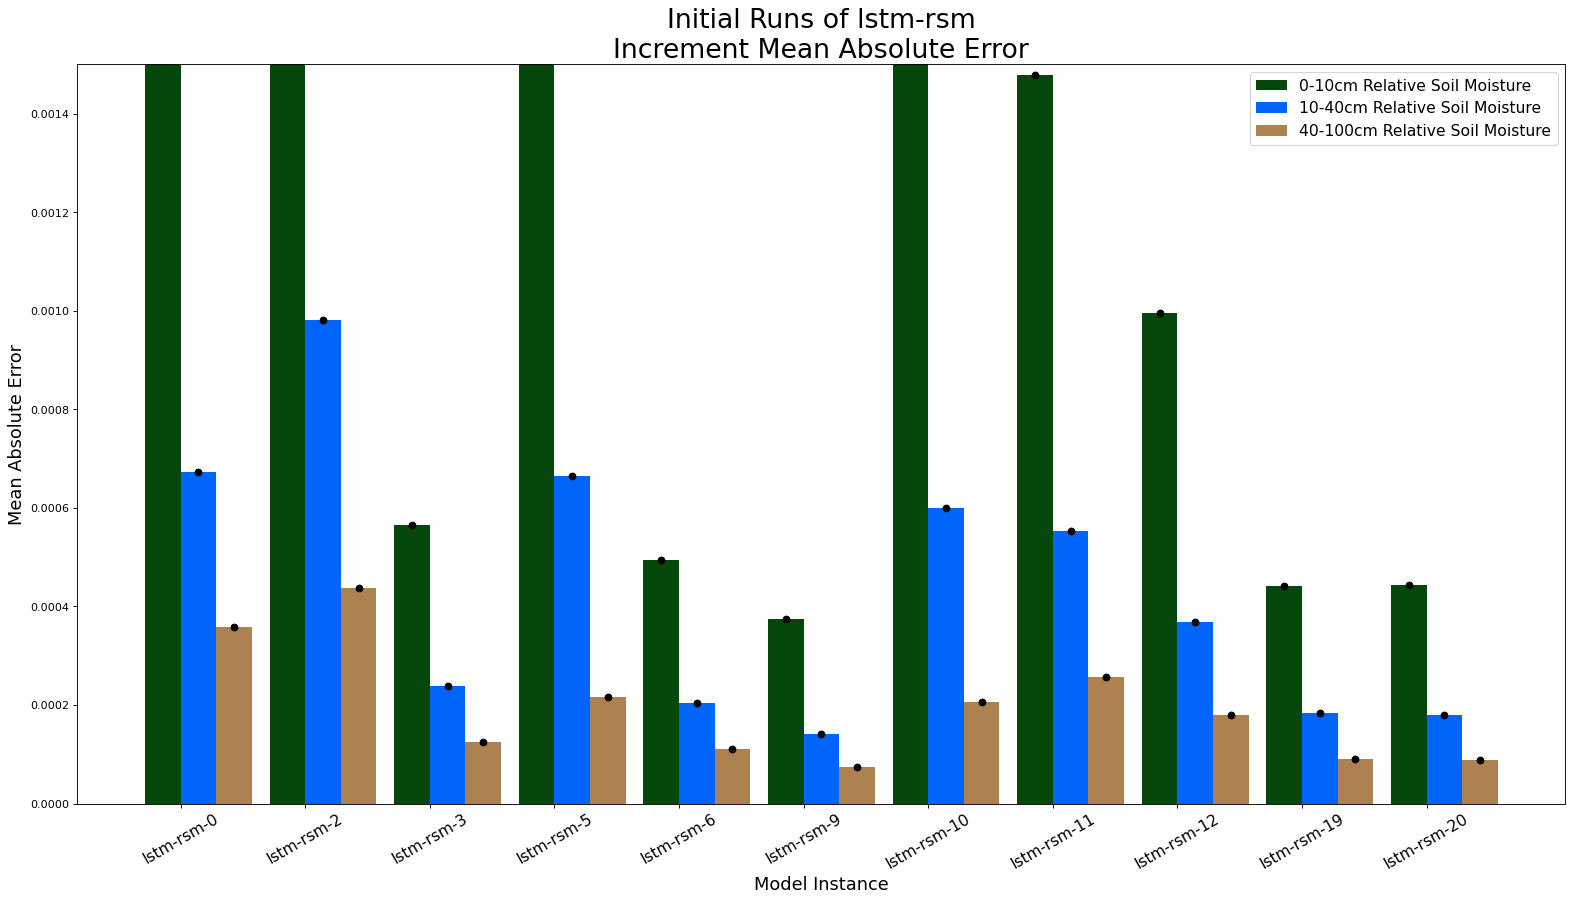
\includegraphics[width=.48\linewidth,draft=false]{figures/efficiency_initial-best/eval_test_efficiency_initial-lstm-rsm_mae_res.png}
    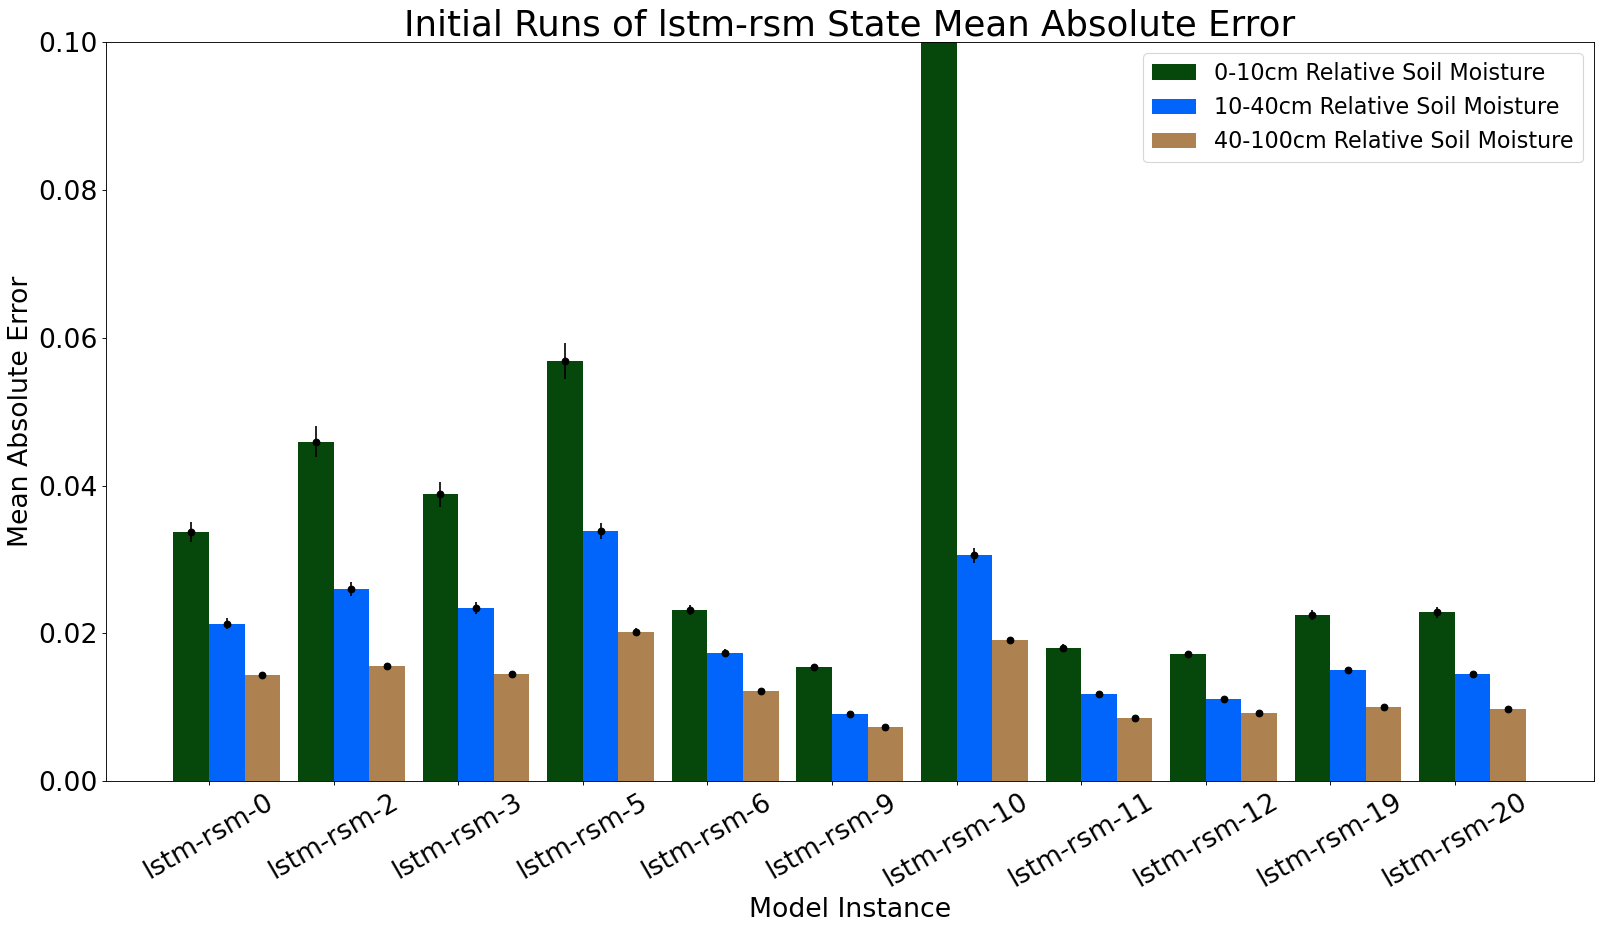
\includegraphics[width=.48\linewidth,draft=false]{figures/efficiency_initial-best/eval_test_efficiency_initial-lstm-rsm_mae_state.png}

    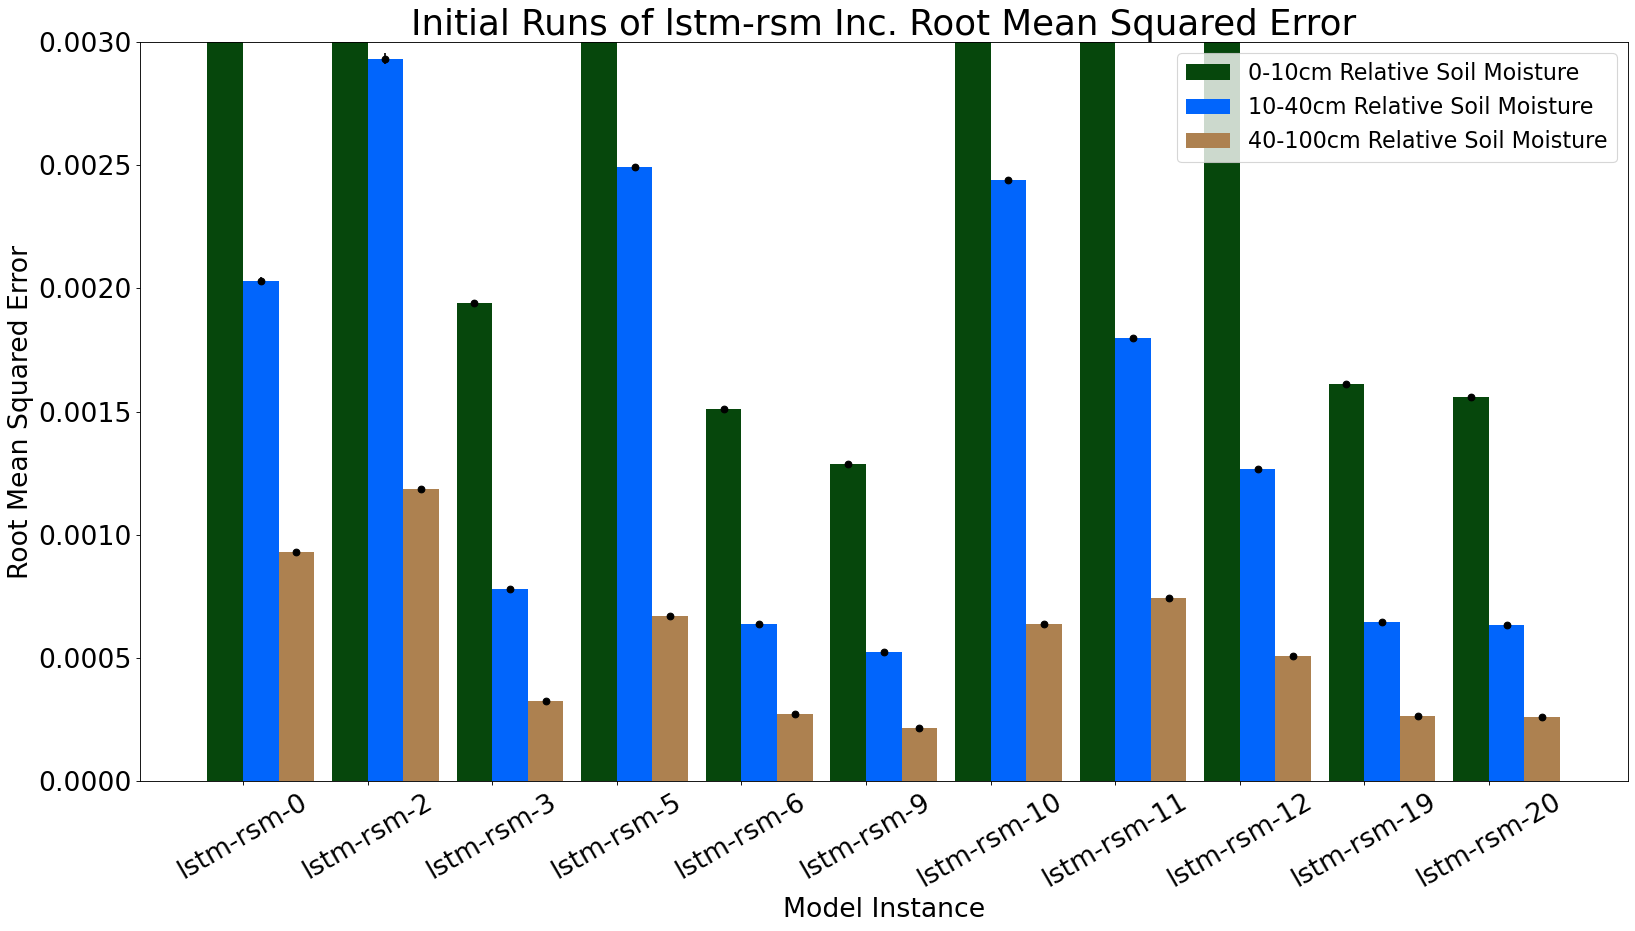
\includegraphics[width=.48\linewidth,draft=false]{figures/efficiency_initial-best/eval_test_efficiency_initial-lstm-rsm_mse_res.png}
    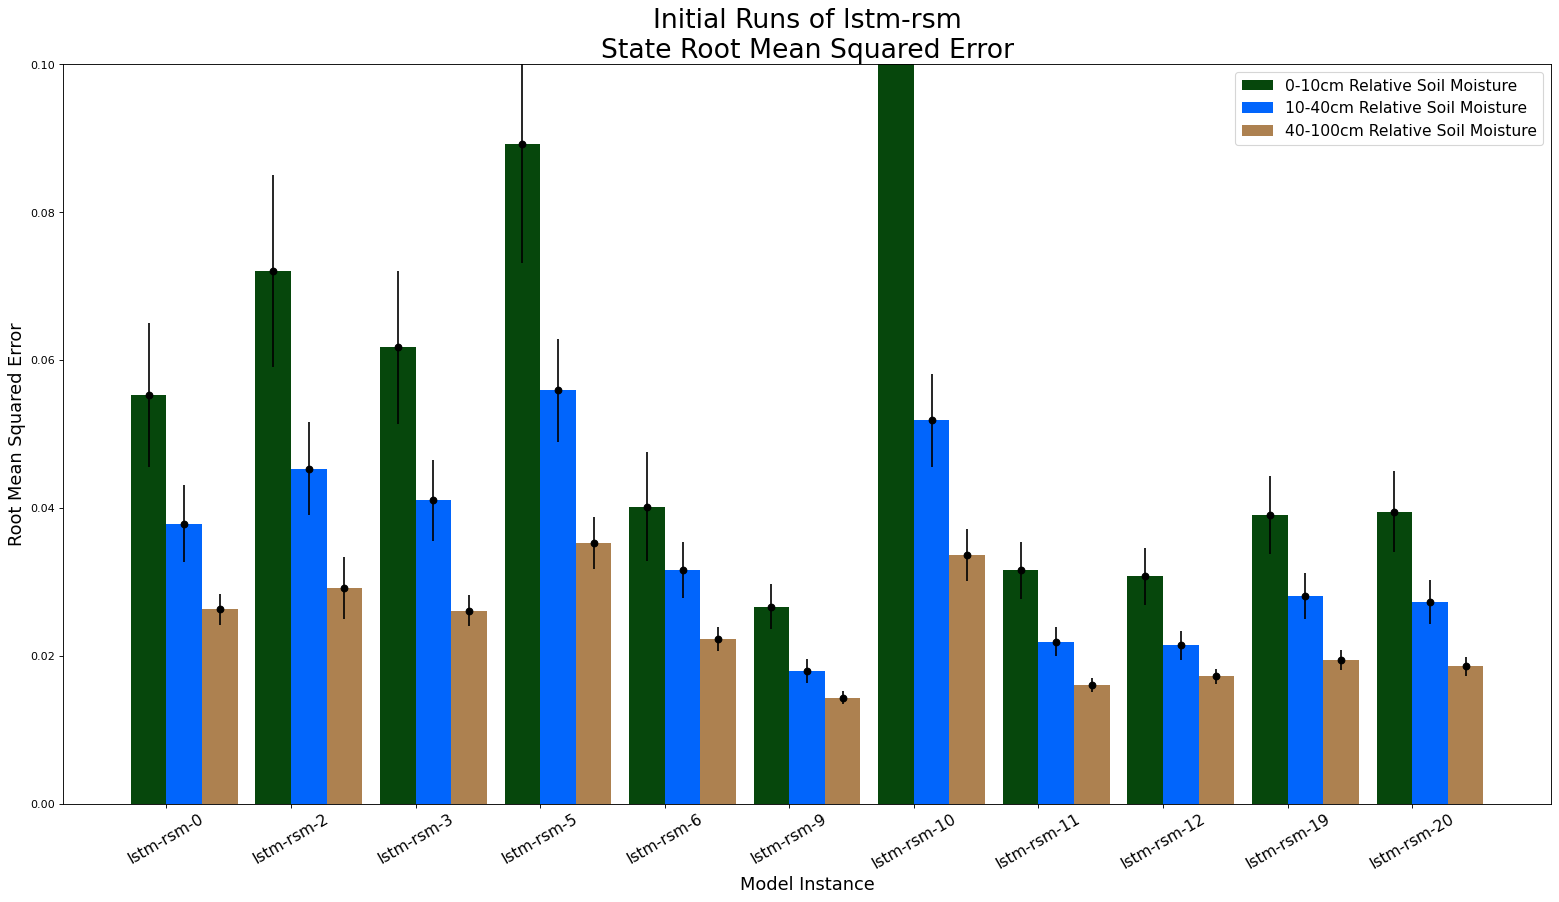
\includegraphics[width=.48\linewidth,draft=false]{figures/efficiency_initial-best/eval_test_efficiency_initial-lstm-rsm_mse_state.png}

    \caption{Bulk metrics for initial LSTM-RSM (relative soil moisture predictor) training runs}
    \label{model-init-lstm-rsm}
\end{figure}

\begin{figure}[hp!]
    \centering
    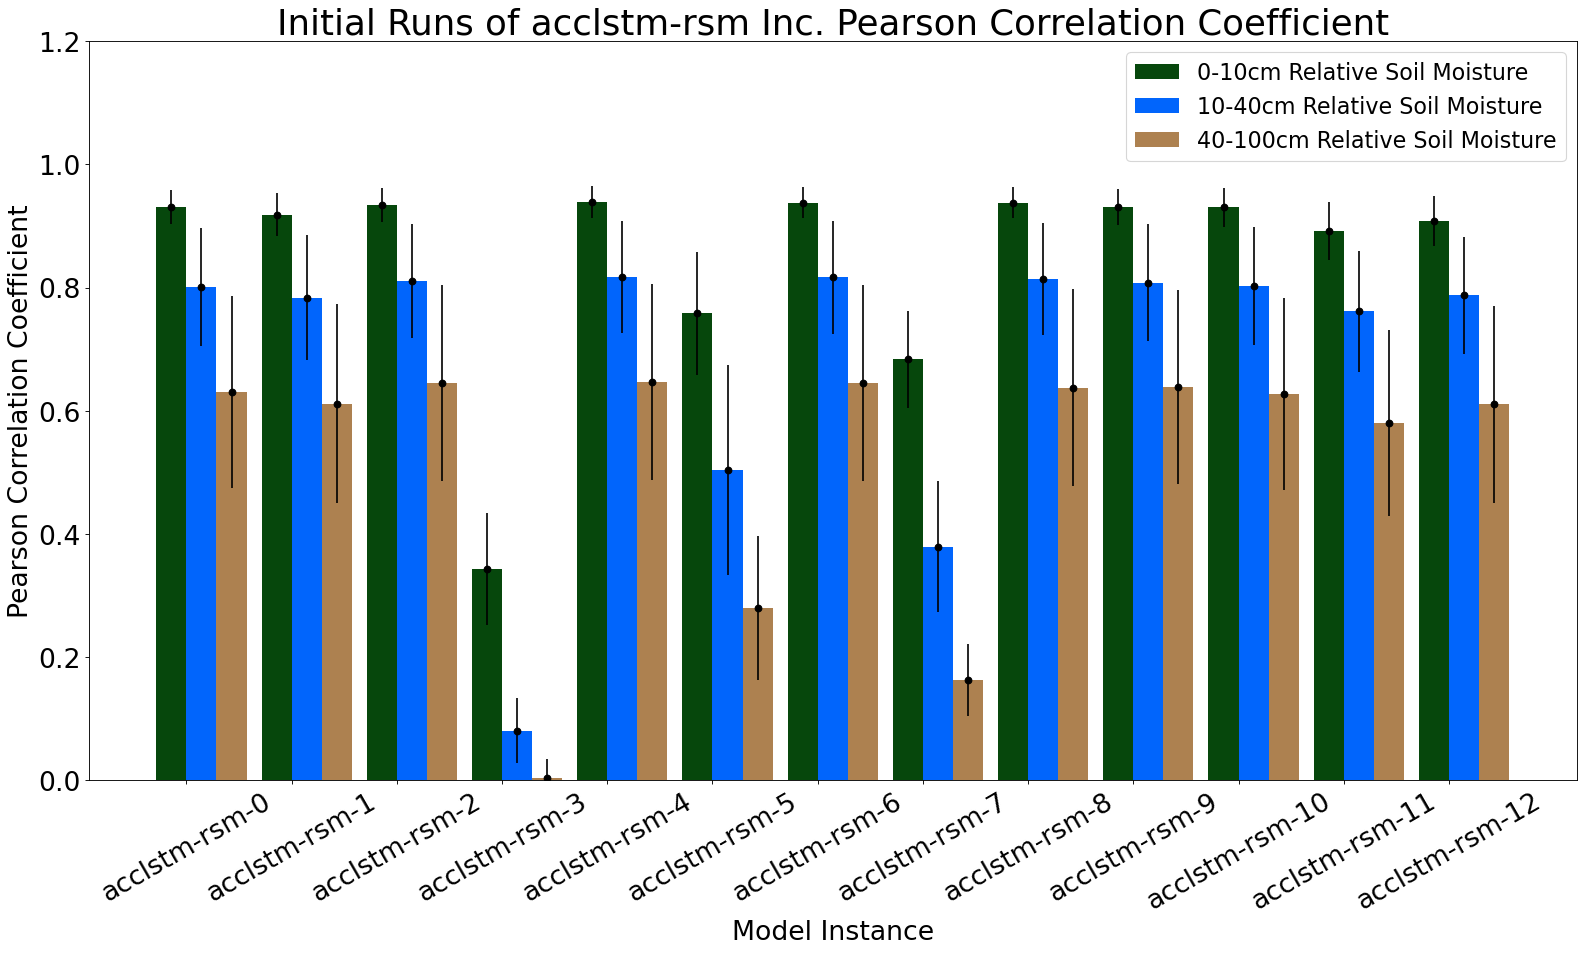
\includegraphics[width=.48\linewidth,draft=false]{figures/efficiency_initial-best/eval_test_efficiency_initial-acclstm-rsm_cc_res.png}
    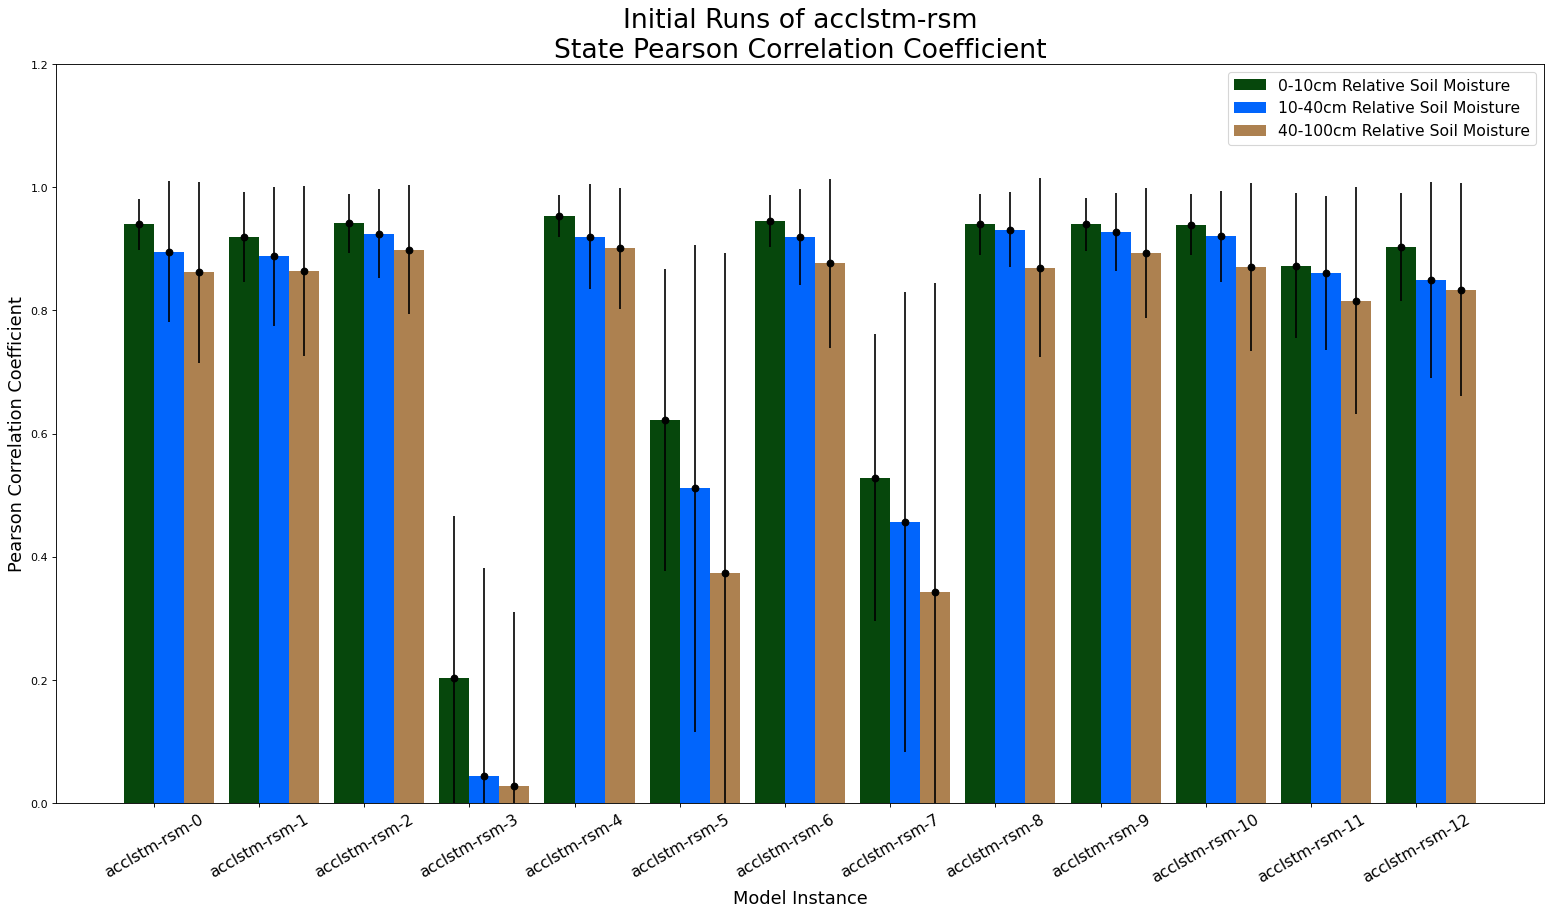
\includegraphics[width=.48\linewidth,draft=false]{figures/efficiency_initial-best/eval_test_efficiency_initial-acclstm-rsm_cc_state.png}

    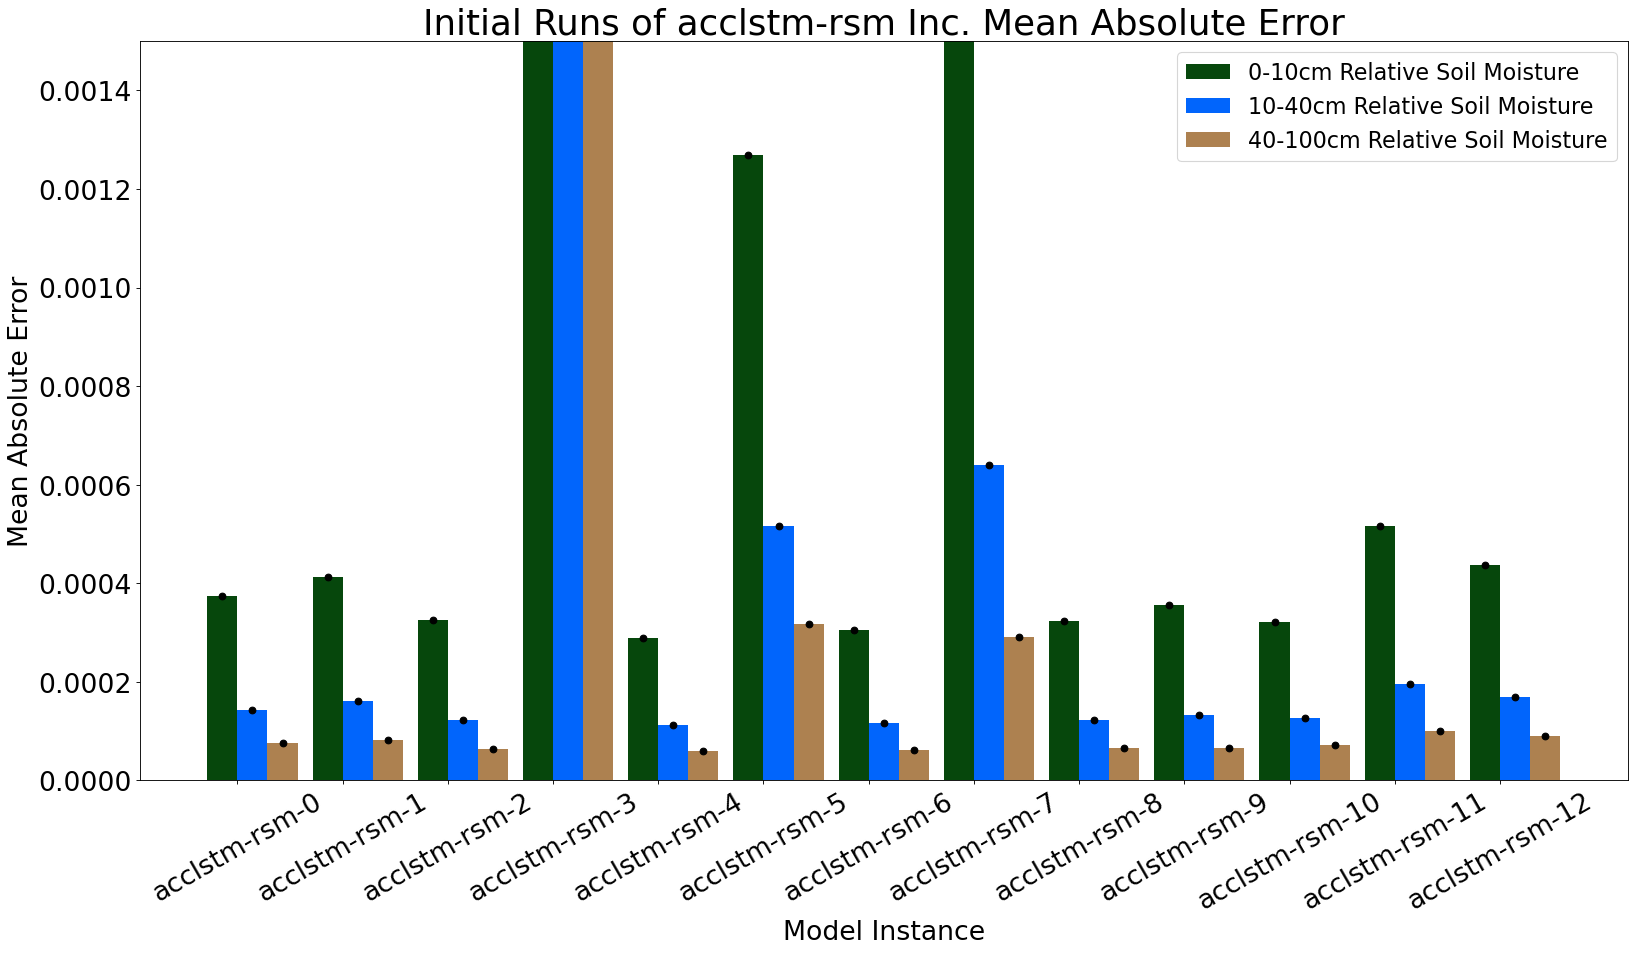
\includegraphics[width=.48\linewidth,draft=false]{figures/efficiency_initial-best/eval_test_efficiency_initial-acclstm-rsm_mae_res.png}
    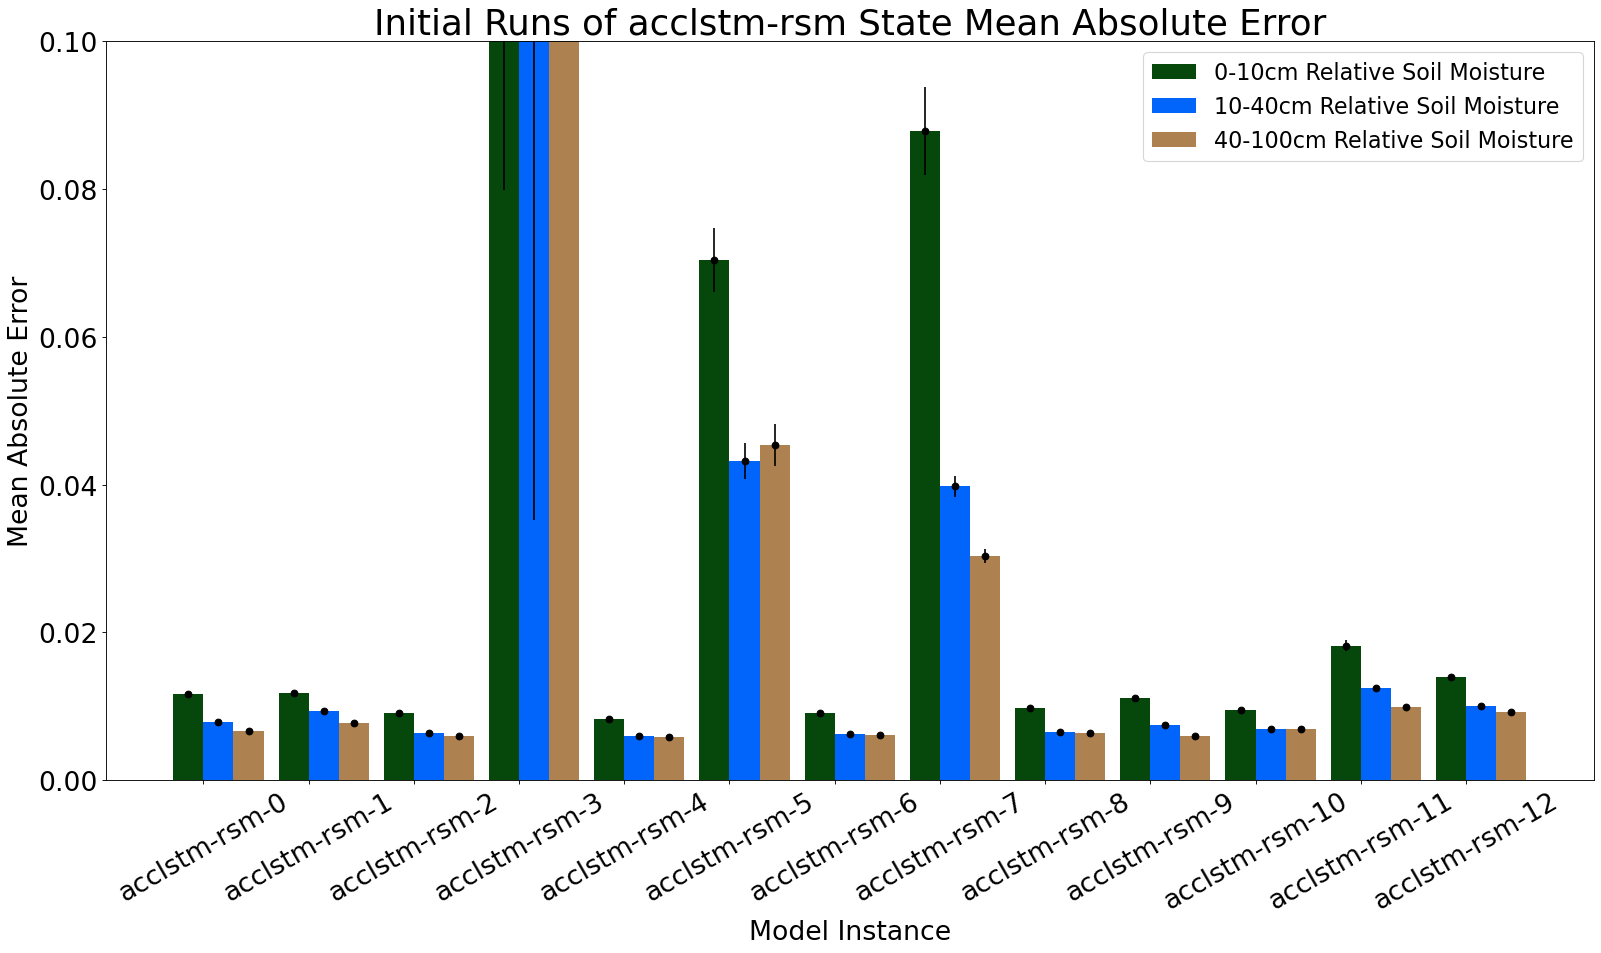
\includegraphics[width=.48\linewidth,draft=false]{figures/efficiency_initial-best/eval_test_efficiency_initial-acclstm-rsm_mae_state.png}

    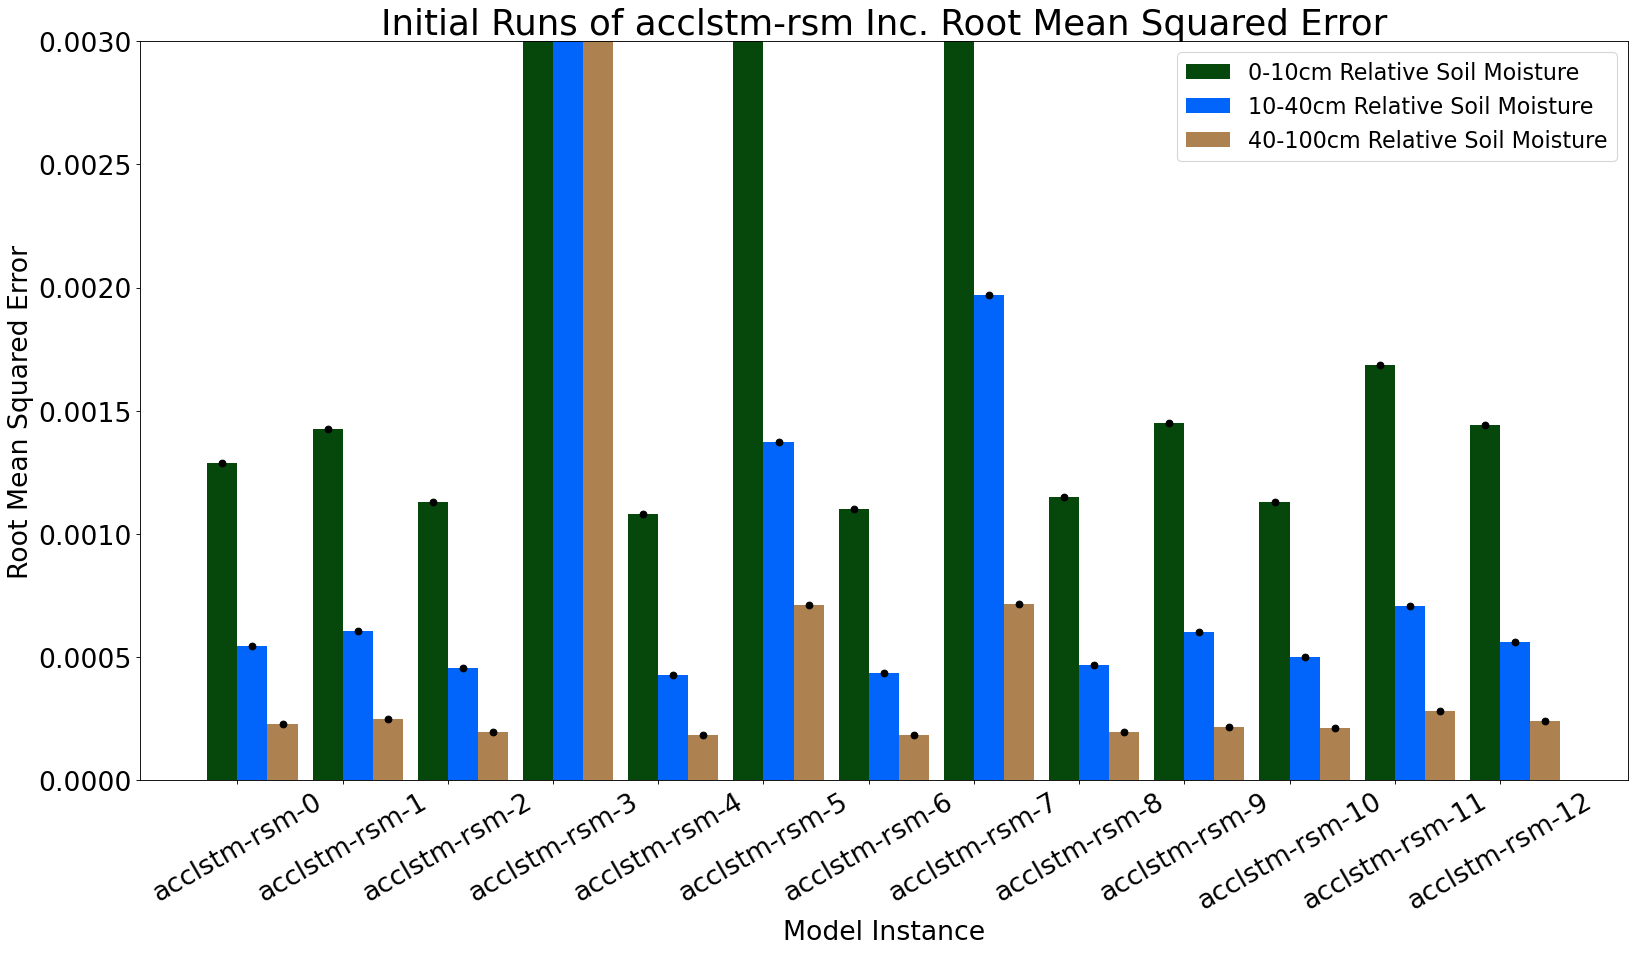
\includegraphics[width=.48\linewidth,draft=false]{figures/efficiency_initial-best/eval_test_efficiency_initial-acclstm-rsm_mse_res.png}
    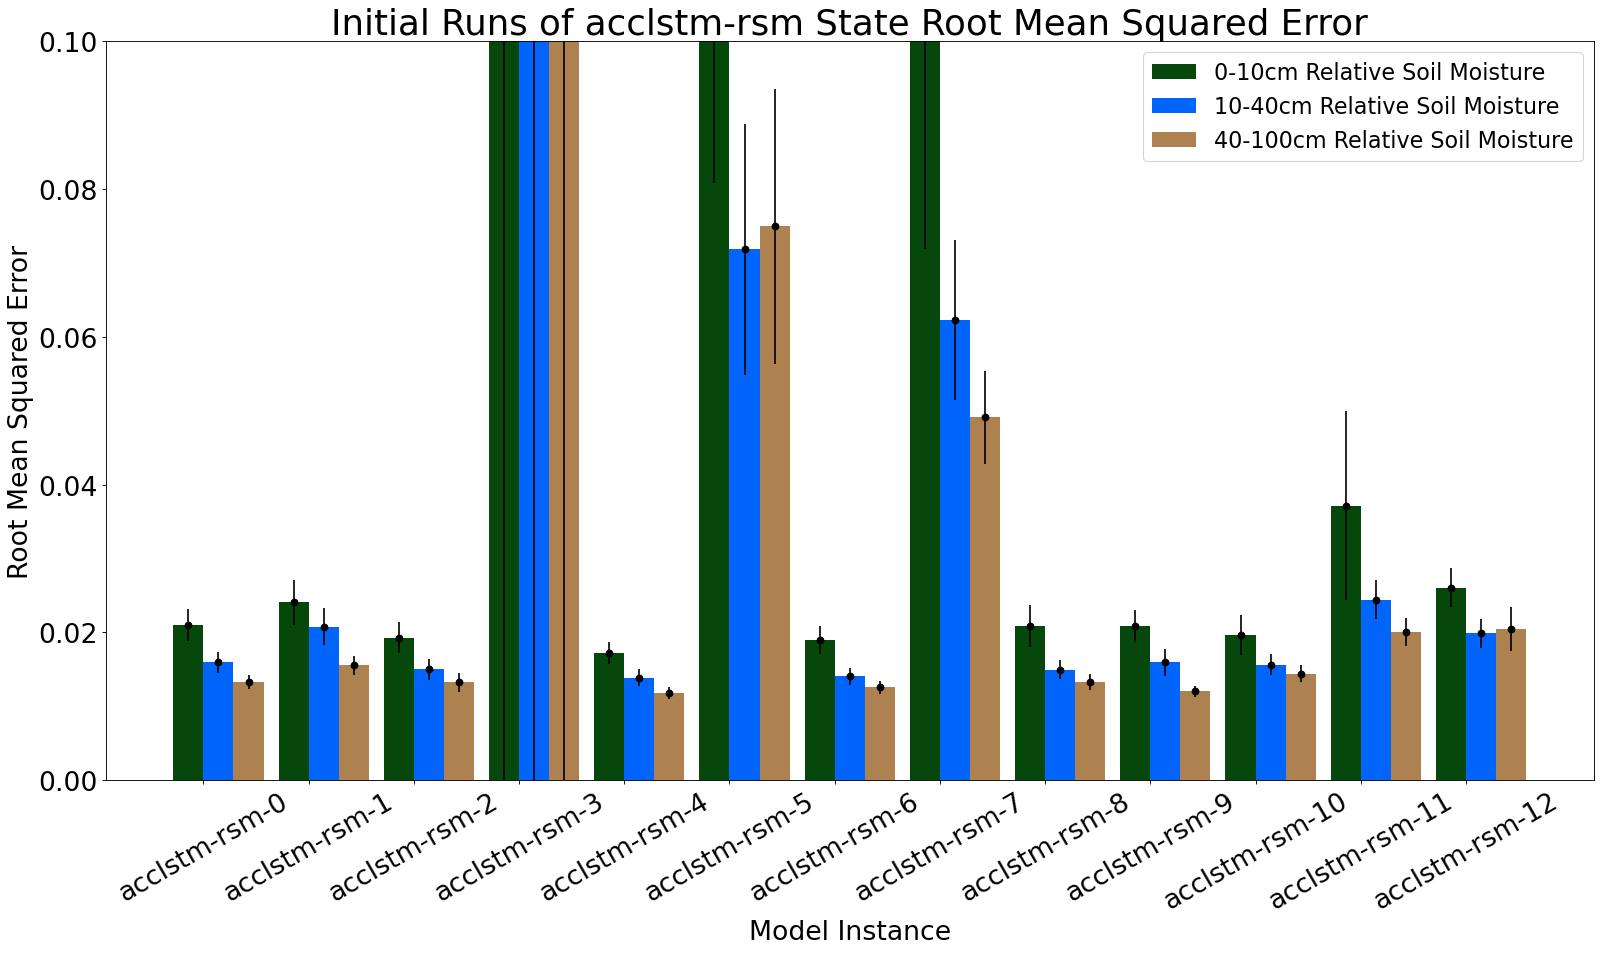
\includegraphics[width=.48\linewidth,draft=false]{figures/efficiency_initial-best/eval_test_efficiency_initial-acclstm-rsm_mse_state.png}

    \caption{Bulk metrics for initial AccLSTM-RSM training runs}
    \label{model-init-acclstm-rsm}
\end{figure}

\section{Best Models' Bulk Statistics Comparison}

\begin{figure}[hp!]
    \centering
    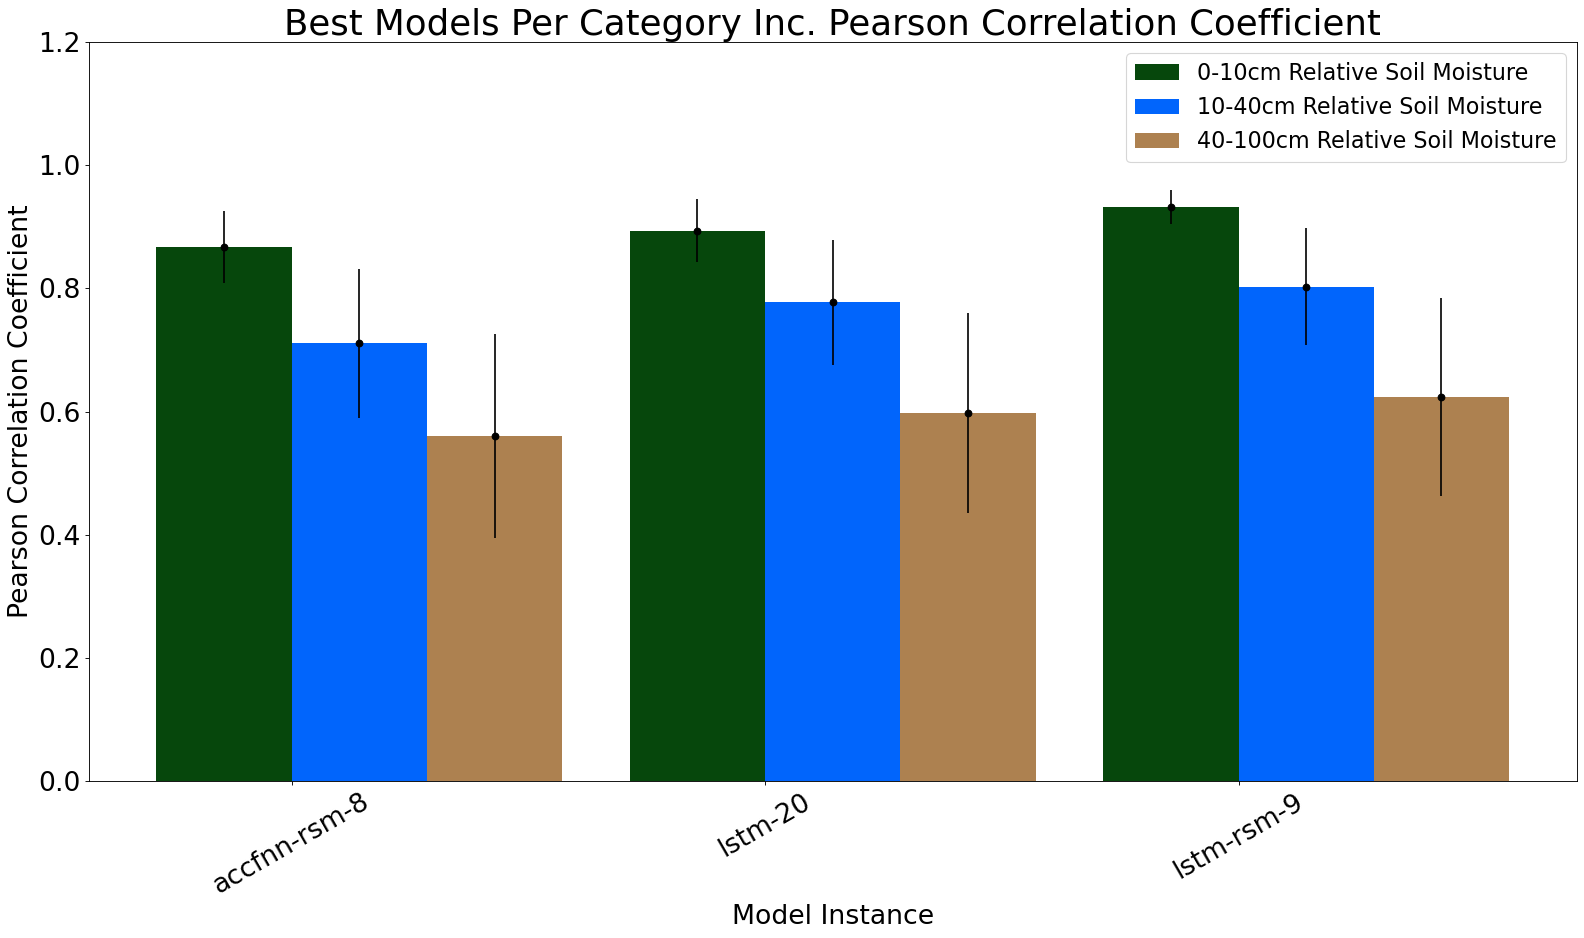
\includegraphics[width=.48\linewidth,draft=false]{figures/efficiency_initial-best/eval_test_efficiency_initial-best_cc_res.png}
    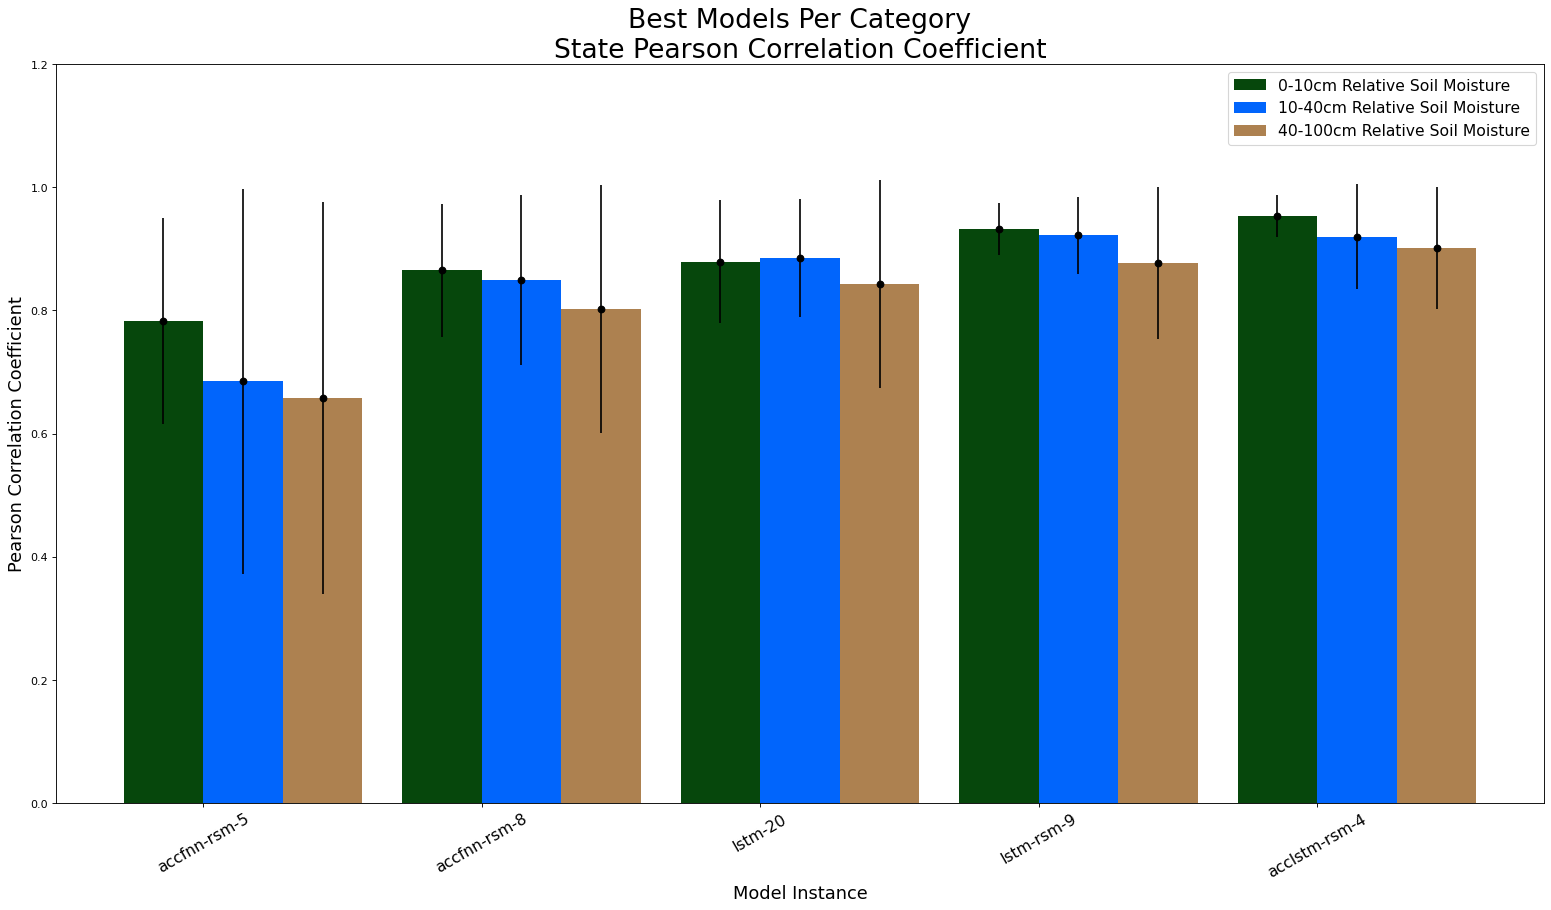
\includegraphics[width=.48\linewidth,draft=false]{figures/efficiency_initial-best/eval_test_efficiency_initial-best_cc_state.png}

    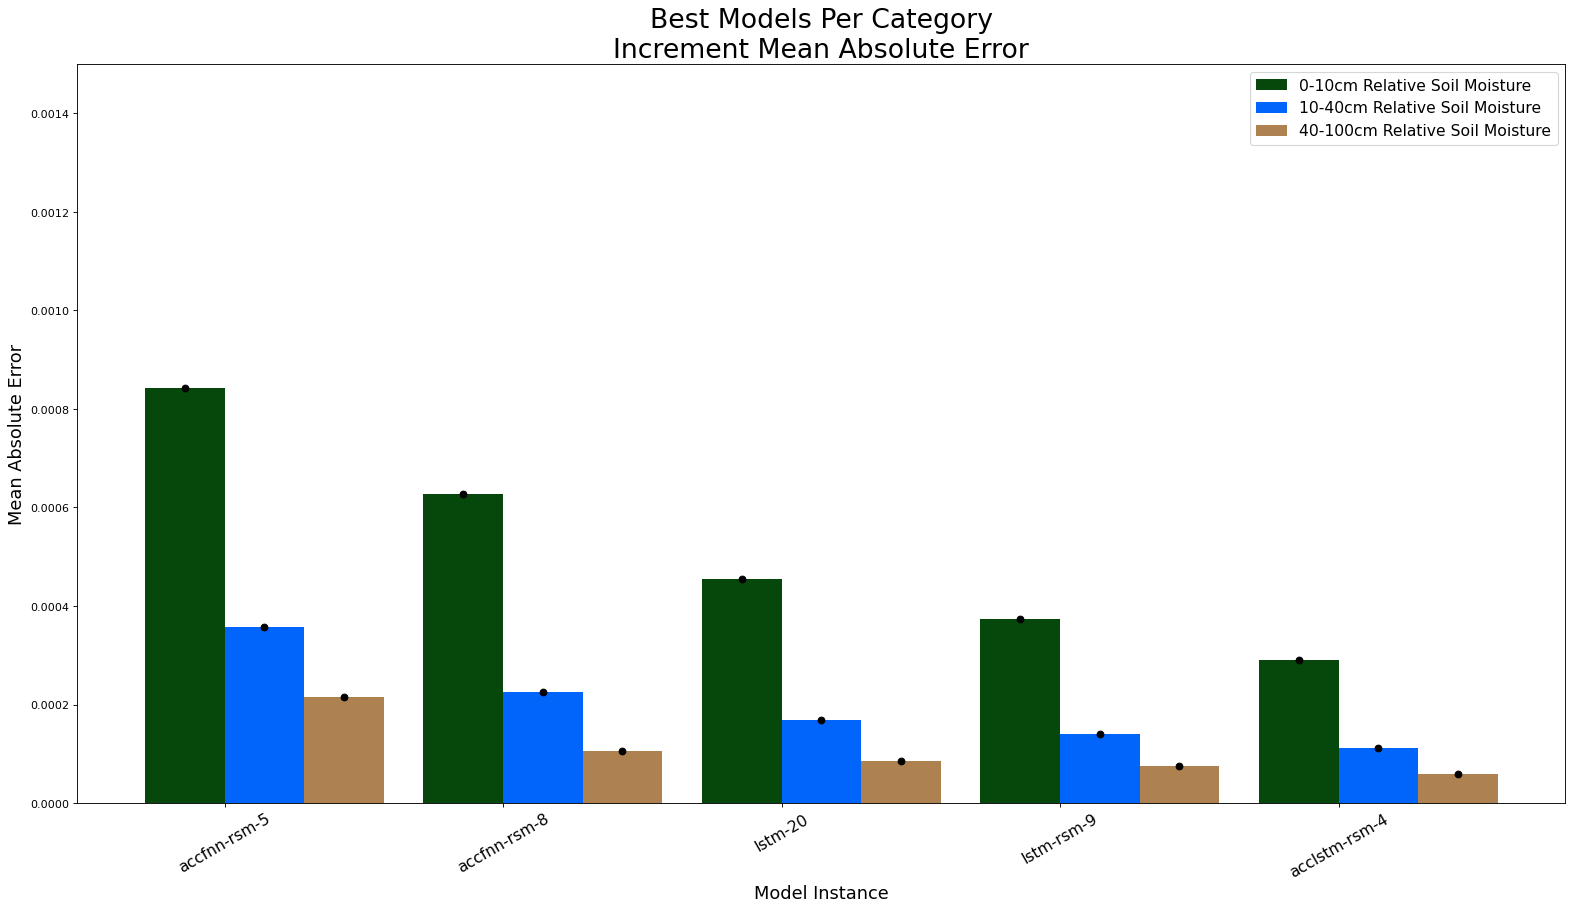
\includegraphics[width=.48\linewidth,draft=false]{figures/efficiency_initial-best/eval_test_efficiency_initial-best_mae_res.png}
    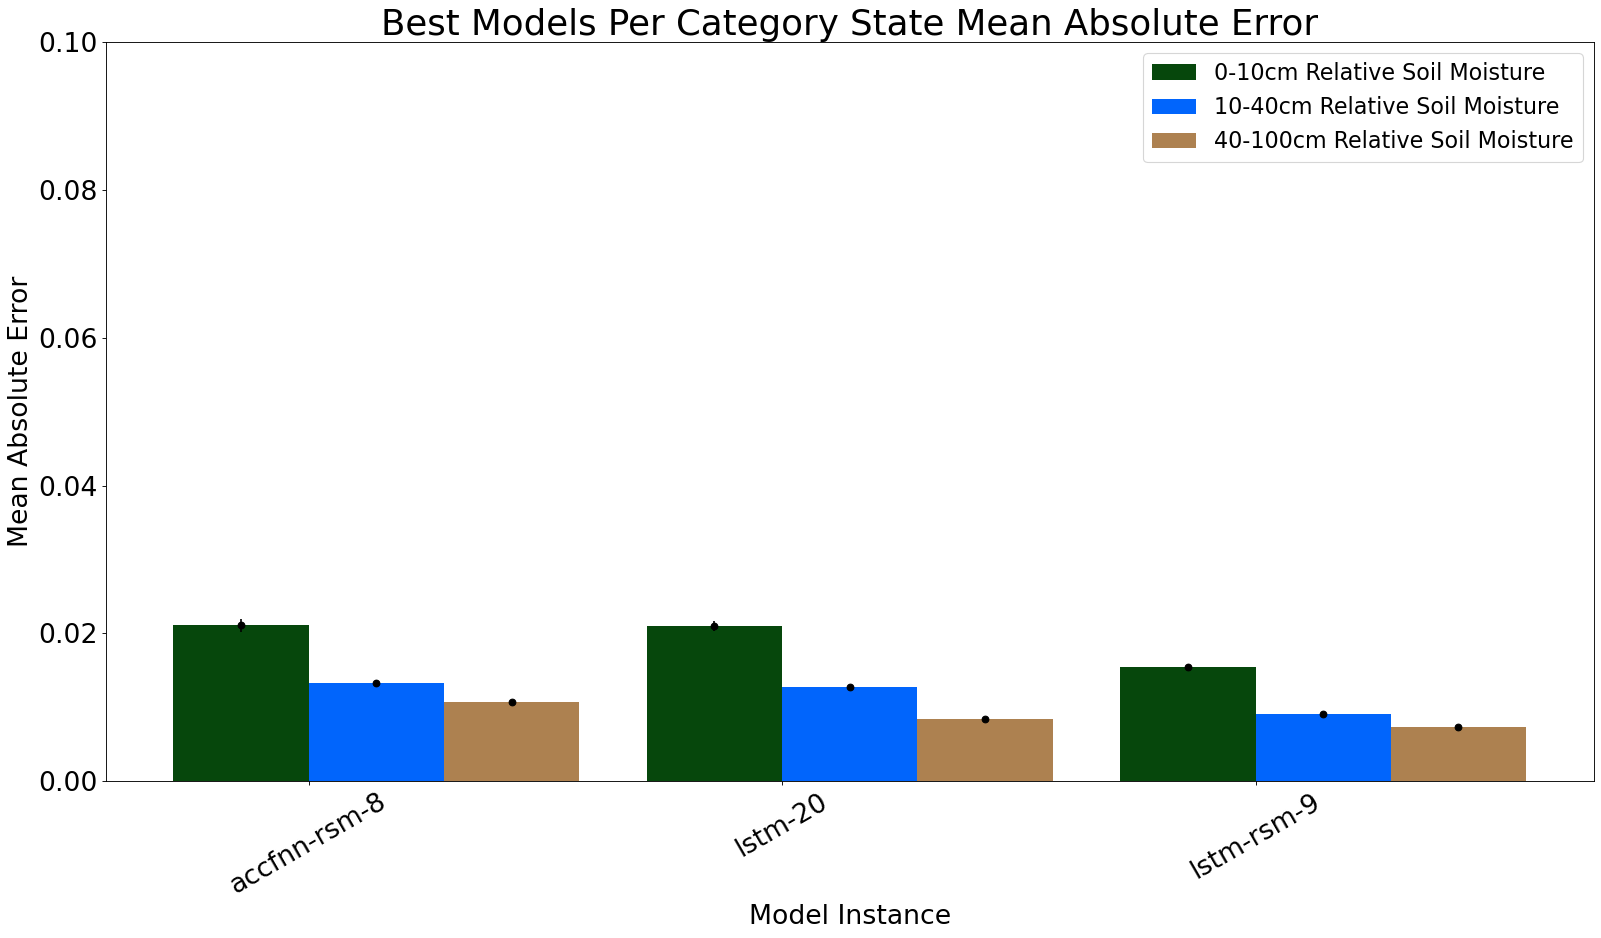
\includegraphics[width=.48\linewidth,draft=false]{figures/efficiency_initial-best/eval_test_efficiency_initial-best_mae_state.png}

    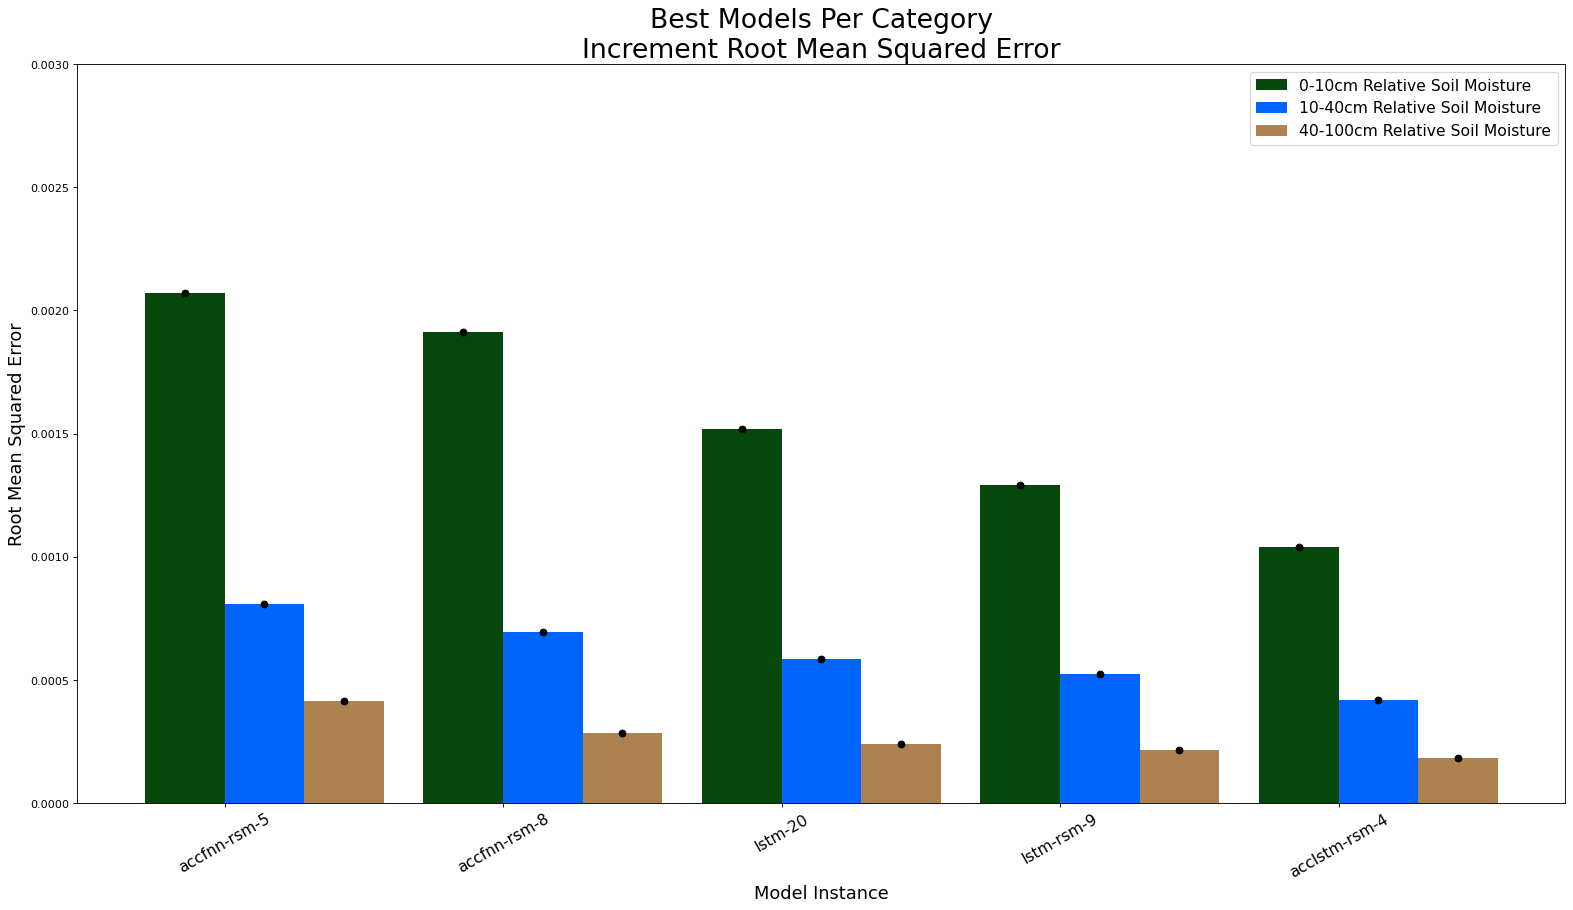
\includegraphics[width=.48\linewidth,draft=false]{figures/efficiency_initial-best/eval_test_efficiency_initial-best_mse_res.png}
    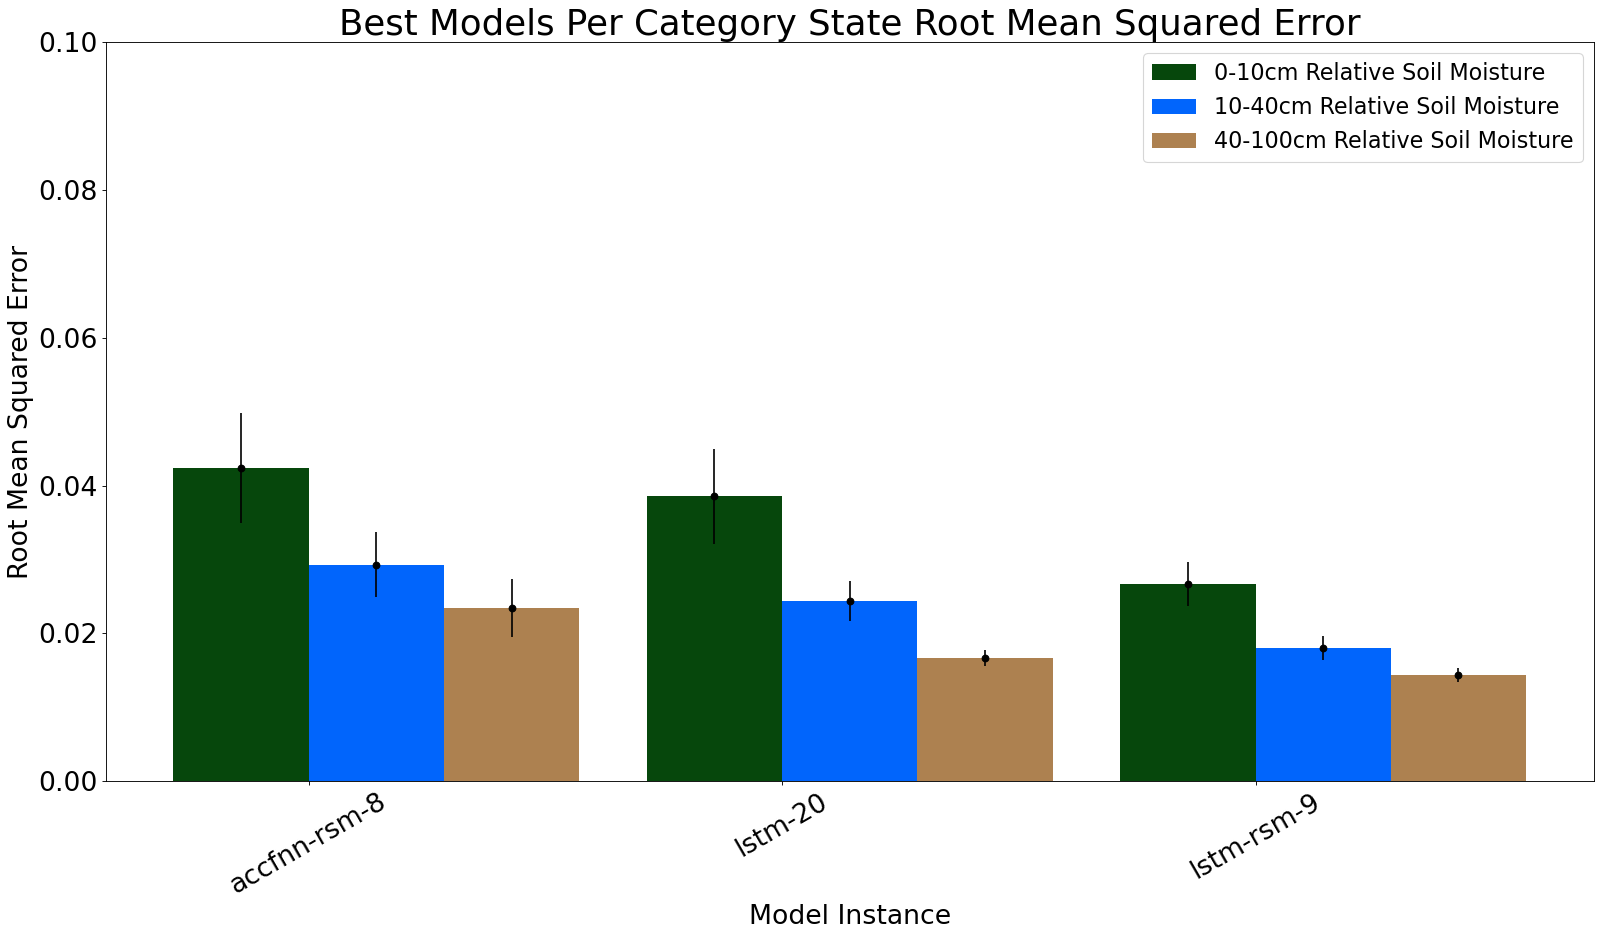
\includegraphics[width=.48\linewidth,draft=false]{figures/efficiency_initial-best/eval_test_efficiency_initial-best_mse_state.png}

    \caption{Bulk metrics comparing the best exploratory models from each category}
    \label{best-metrics}
\end{figure}

\begin{figure}[hp!]
    \centering

    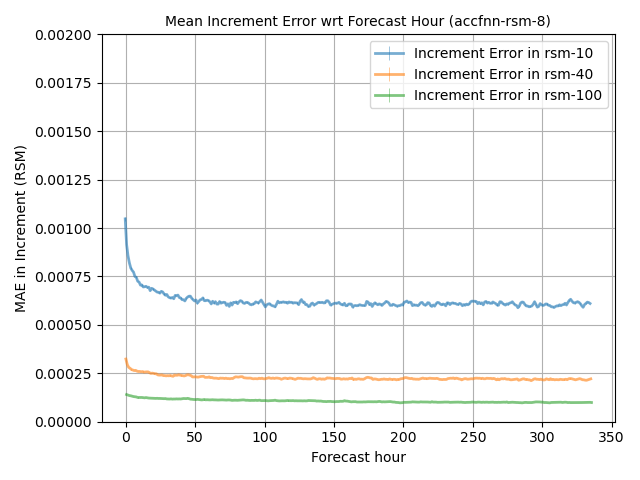
\includegraphics[width=.42\linewidth,draft=false]{figures/horizons/eval_test_accfnn-rsm-8_rsm_horizon_na_res.png}
    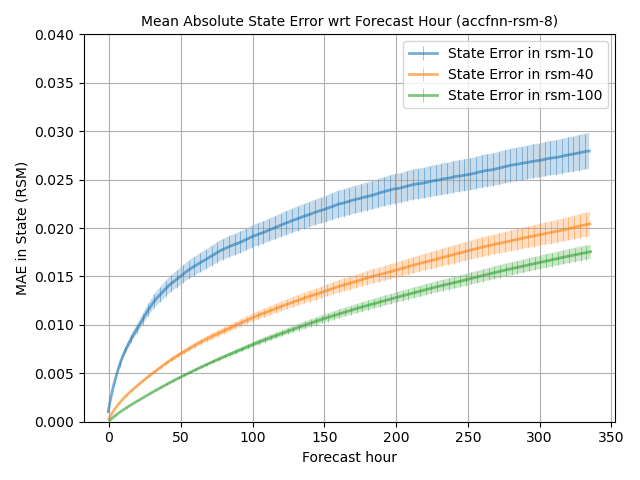
\includegraphics[width=.42\linewidth,draft=false]{figures/horizons/eval_test_accfnn-rsm-8_rsm_horizon_na_state.png}

    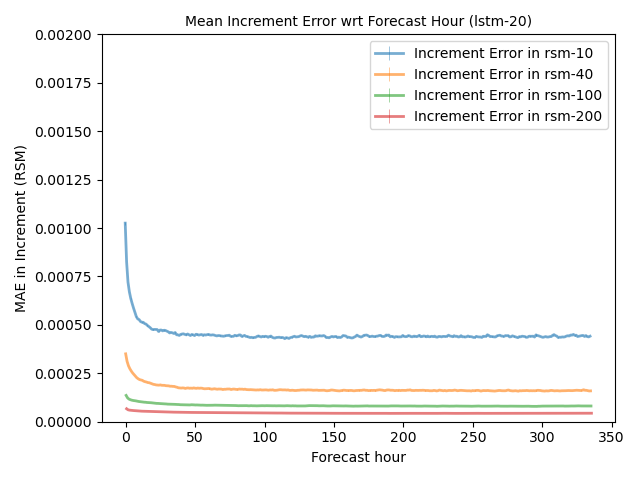
\includegraphics[width=.42\linewidth,draft=false]{figures/horizons/eval_test_lstm-20_rsm_horizon_na_res.png}
    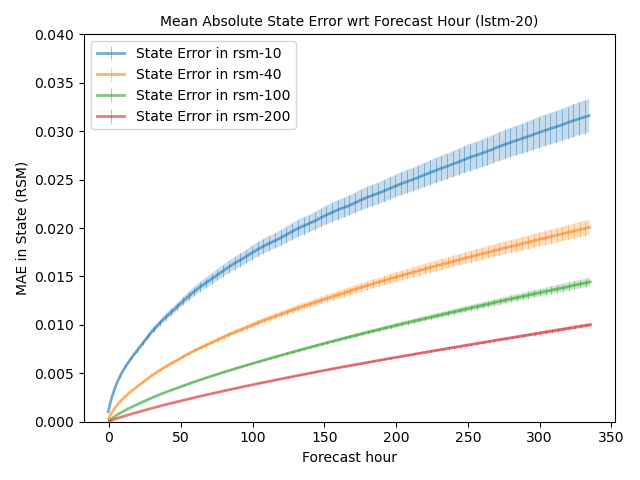
\includegraphics[width=.42\linewidth,draft=false]{figures/horizons/eval_test_lstm-20_rsm_horizon_na_state.png}

    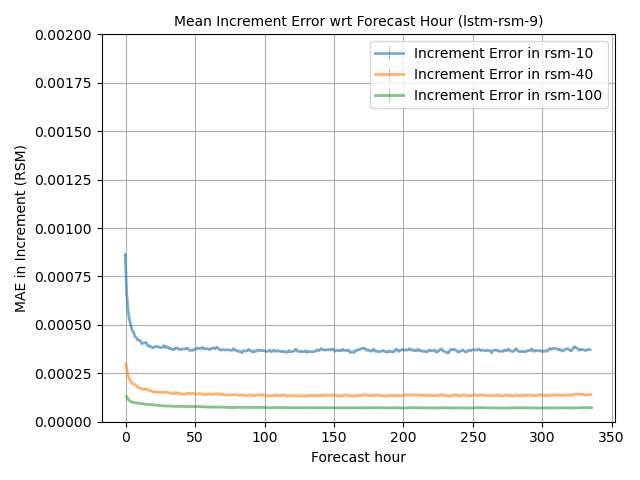
\includegraphics[width=.42\linewidth,draft=false]{figures/horizons/eval_test_lstm-rsm-9_rsm_horizon_na_res.png}
    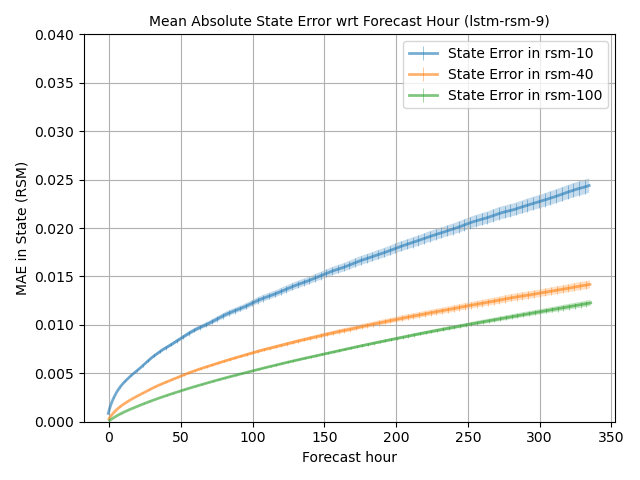
\includegraphics[width=.42\linewidth,draft=false]{figures/horizons/eval_test_lstm-rsm-9_rsm_horizon_na_state.png}

    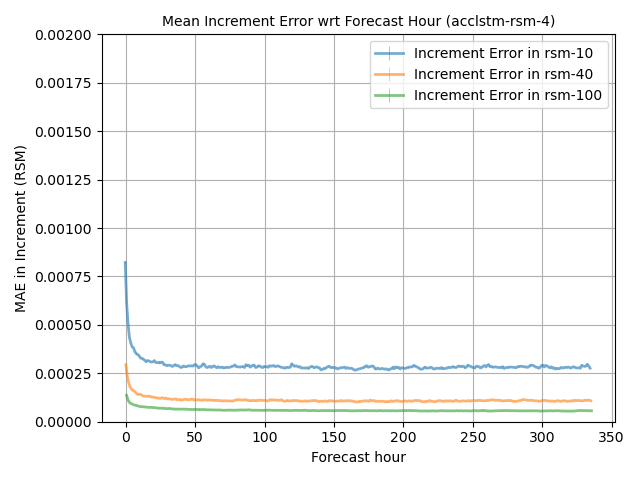
\includegraphics[width=.42\linewidth,draft=false]{figures/horizons/eval_test_acclstm-rsm-4_rsm_horizon_na_res.png}
    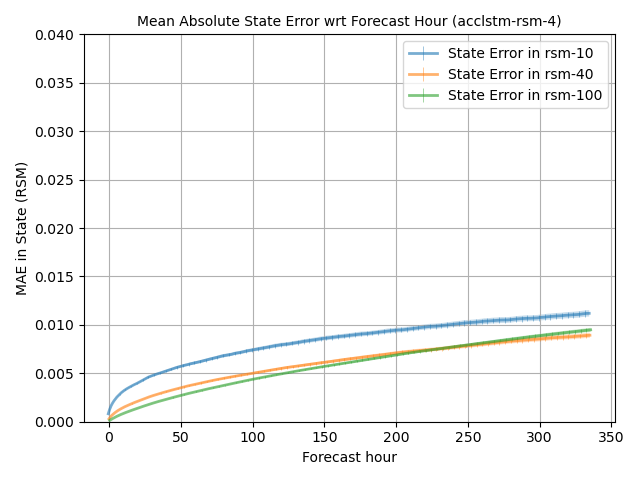
\includegraphics[width=.42\linewidth,draft=false]{figures/horizons/eval_test_acclstm-rsm-4_rsm_horizon_na_state.png}

    \caption{Mean absolute error of each model type with respect to forecast horizon increment (left) and state (right)}
    \label{best-horizons}
\end{figure}

\begin{figure}[hp!]
    \centering

    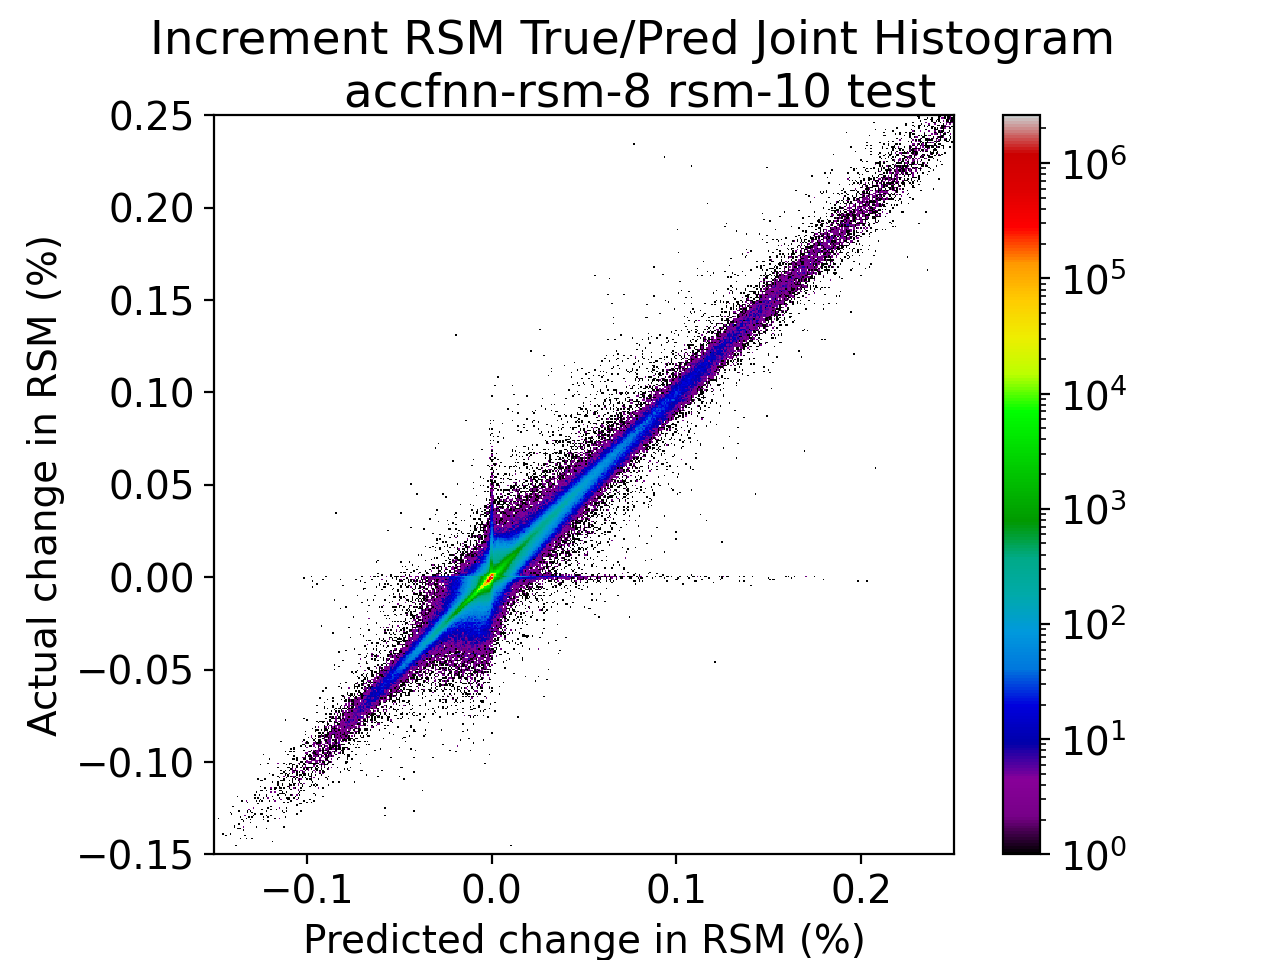
\includegraphics[width=.32\linewidth,draft=false]{figures/validation-curves/eval_test_accfnn-rsm-8_rsm-10_hist-true-pred_na.png}
    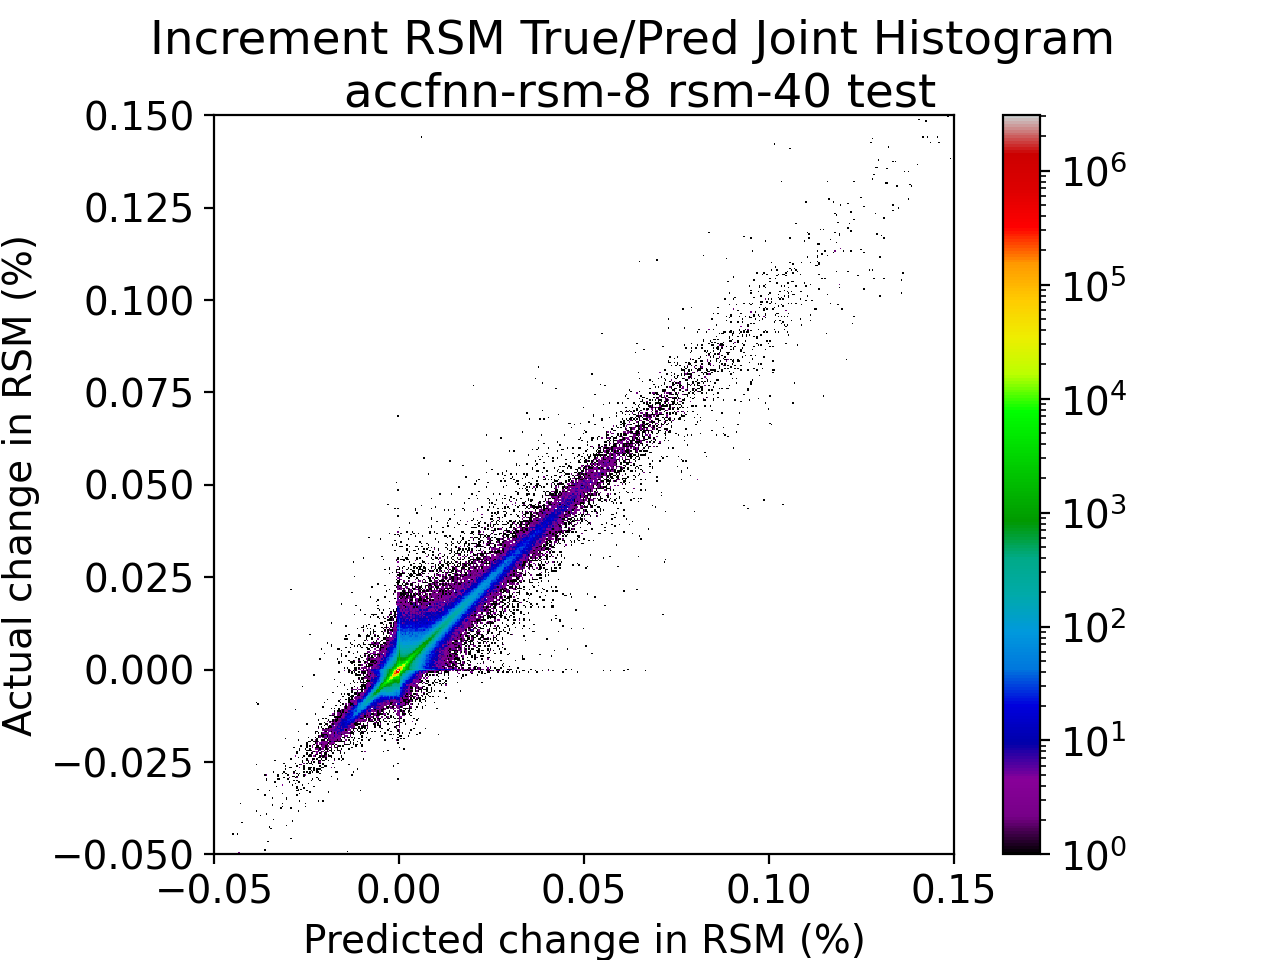
\includegraphics[width=.32\linewidth,draft=false]{figures/validation-curves/eval_test_accfnn-rsm-8_rsm-40_hist-true-pred_na.png}
    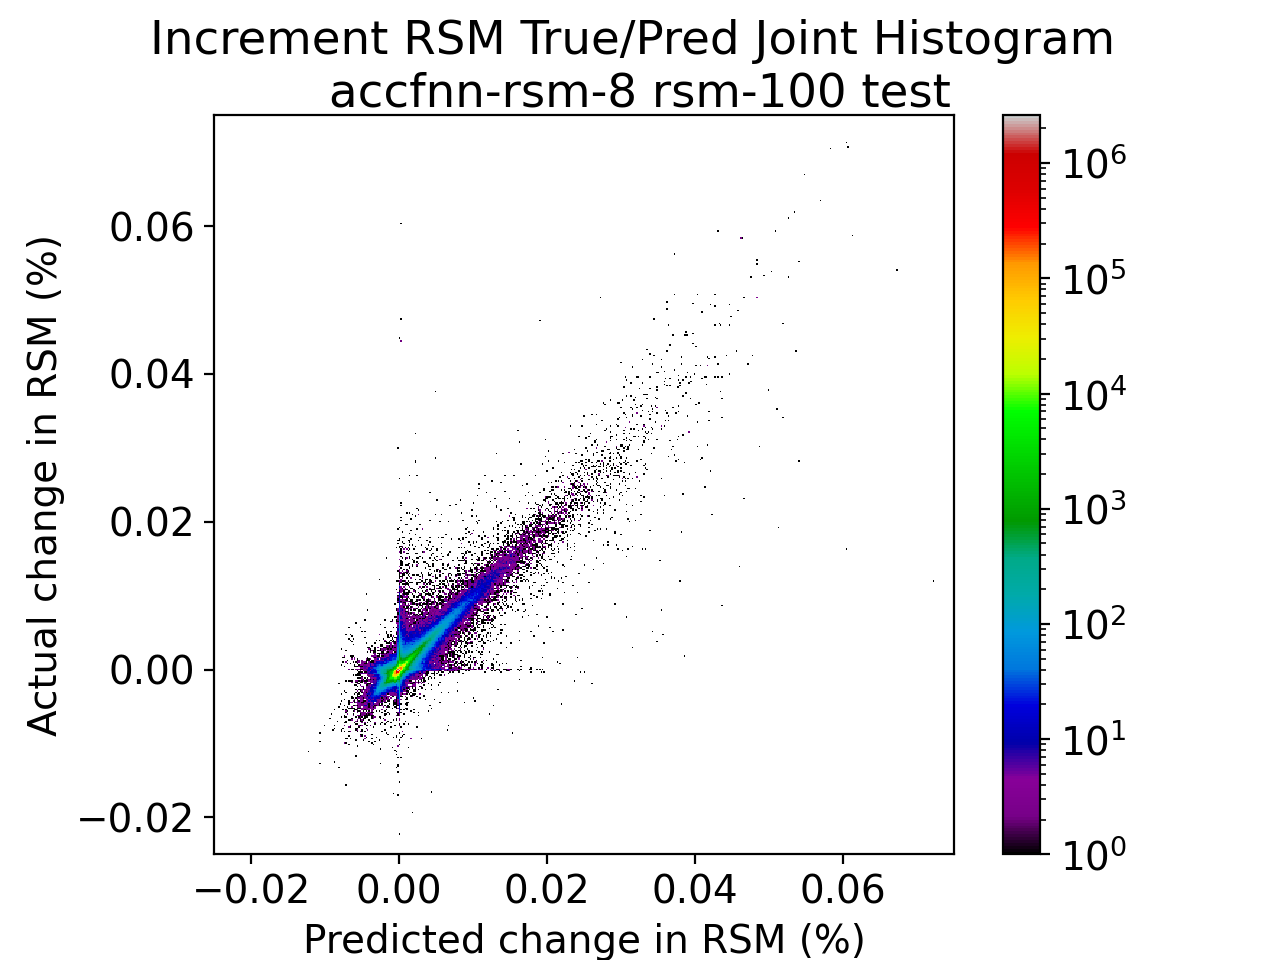
\includegraphics[width=.32\linewidth,draft=false]{figures/validation-curves/eval_test_accfnn-rsm-8_rsm-100_hist-true-pred_na.png}

    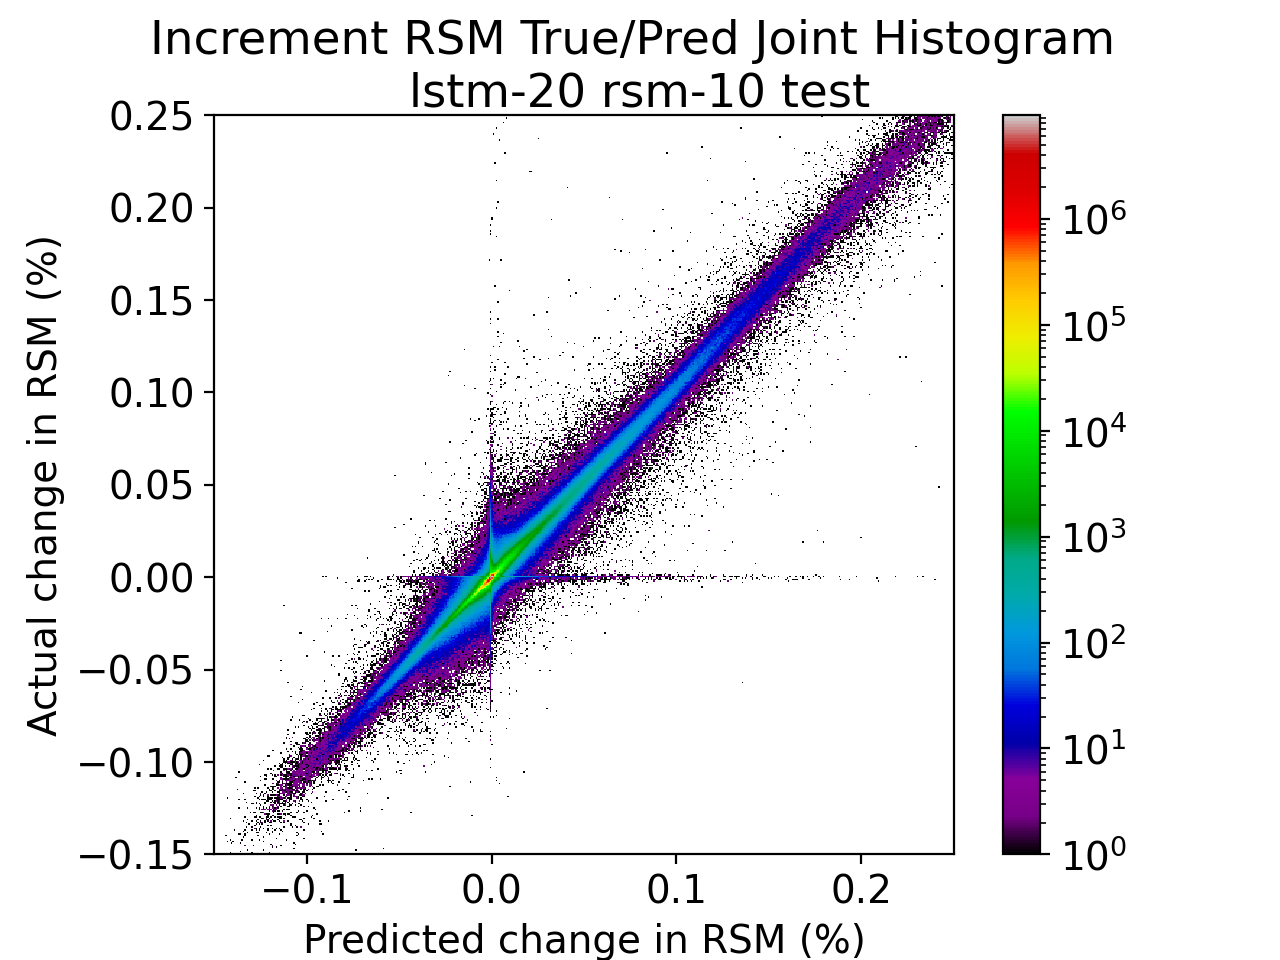
\includegraphics[width=.32\linewidth,draft=false]{figures/validation-curves/eval_test_lstm-20_rsm-10_hist-true-pred_na.png}
    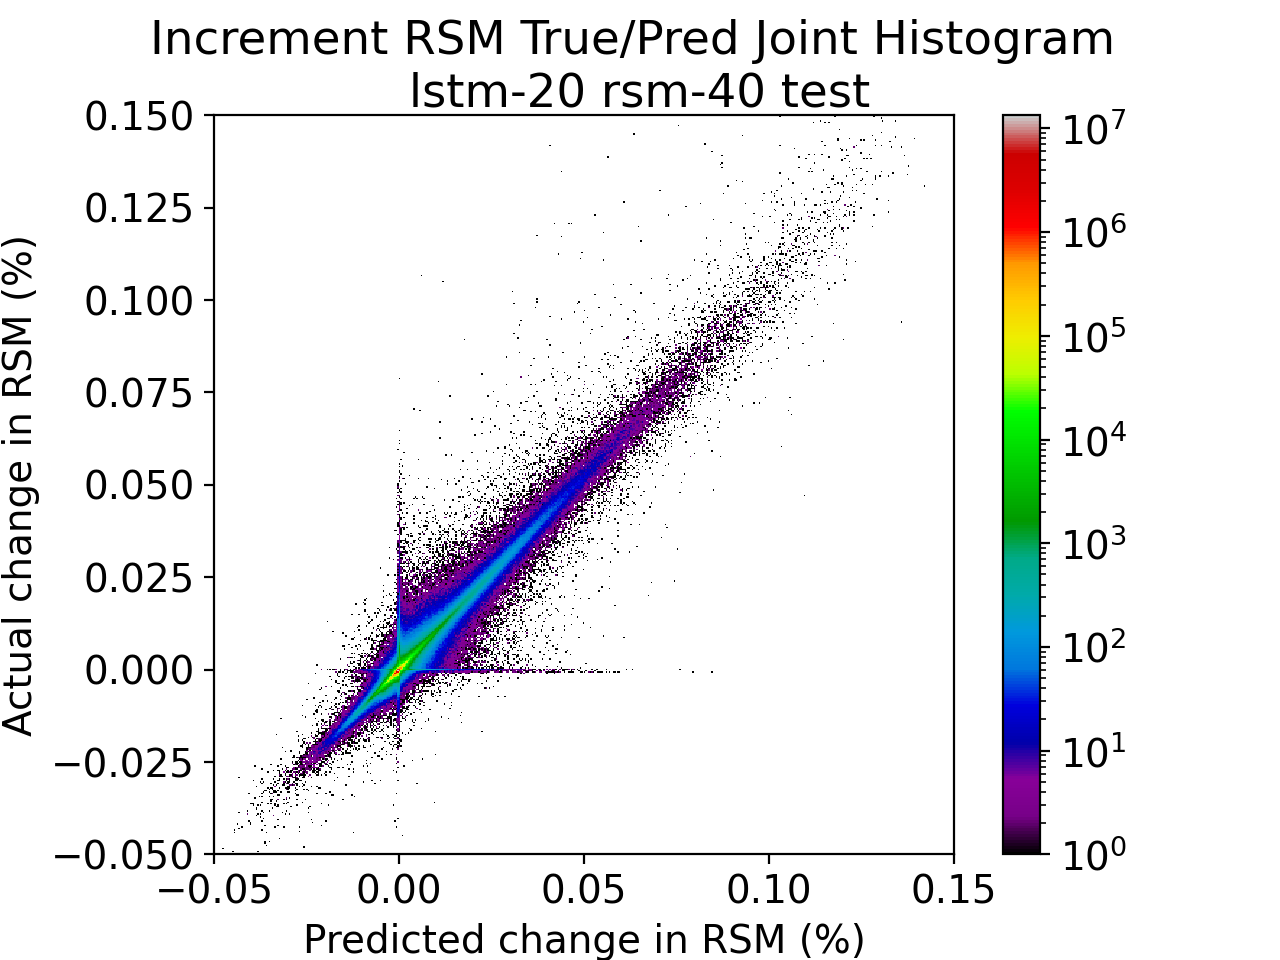
\includegraphics[width=.32\linewidth,draft=false]{figures/validation-curves/eval_test_lstm-20_rsm-40_hist-true-pred_na.png}
    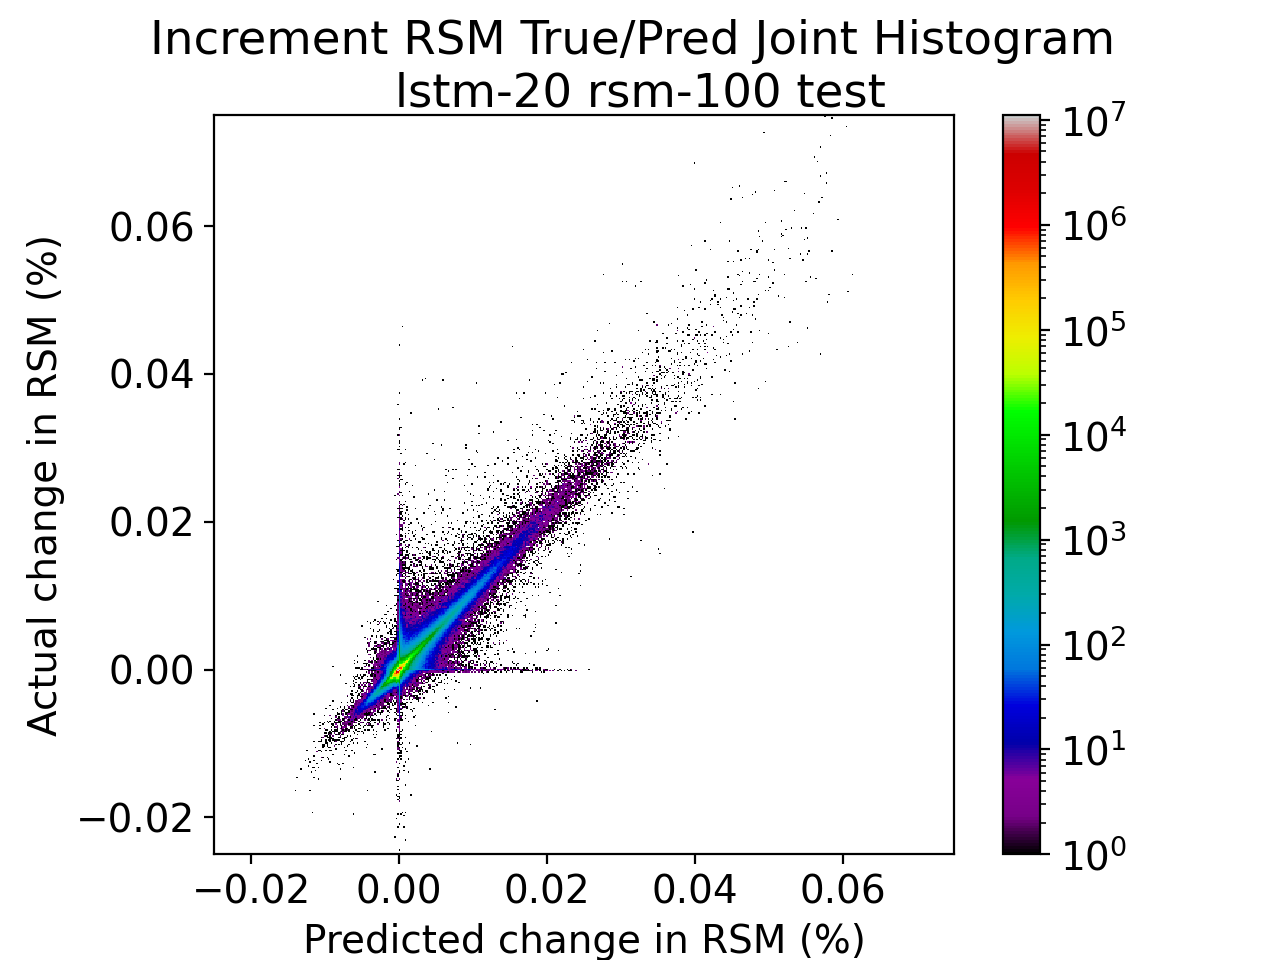
\includegraphics[width=.32\linewidth,draft=false]{figures/validation-curves/eval_test_lstm-20_rsm-100_hist-true-pred_na.png}

    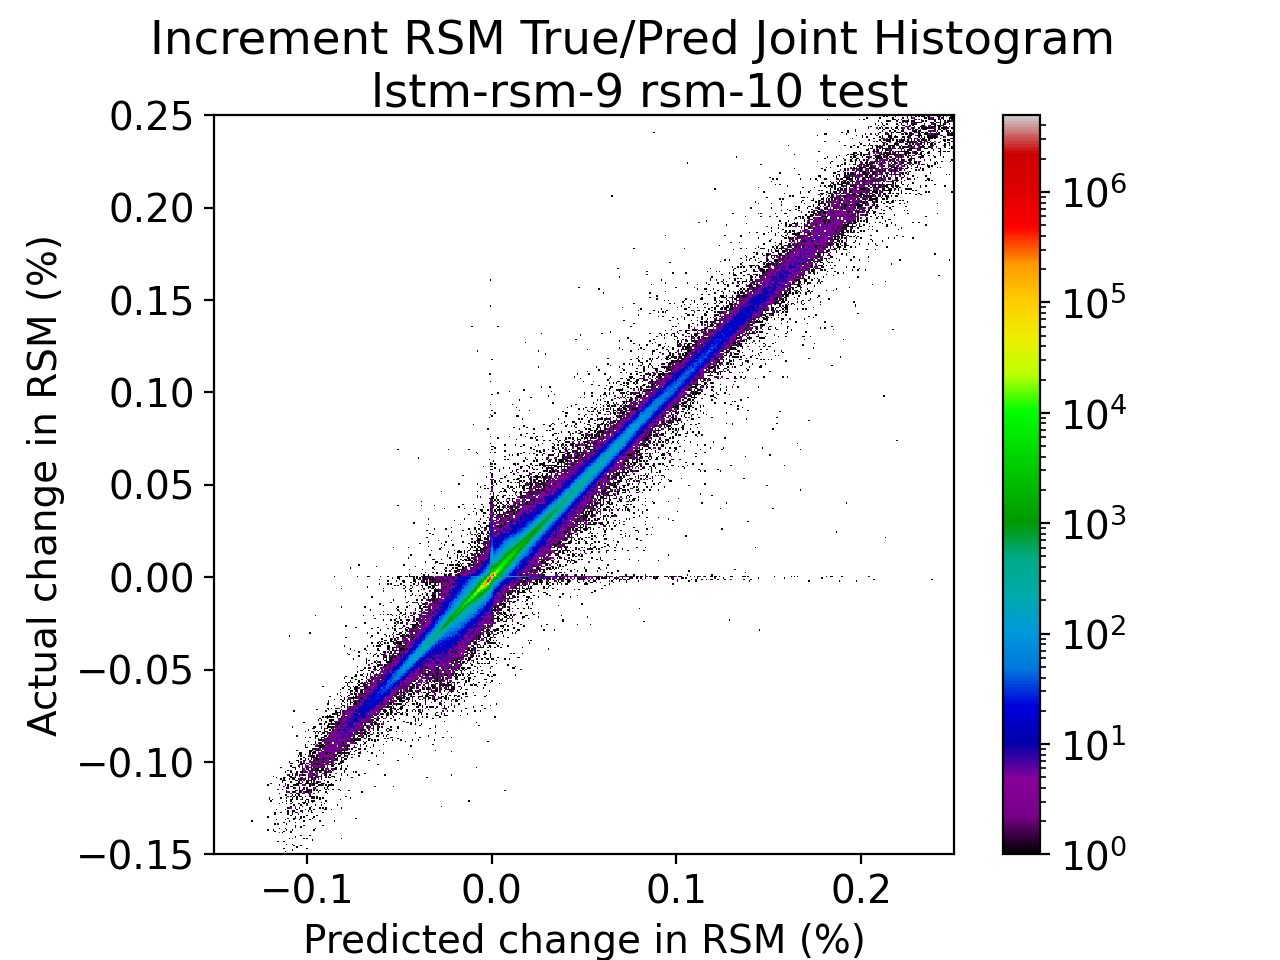
\includegraphics[width=.32\linewidth,draft=false]{figures/validation-curves/eval_test_lstm-rsm-9_rsm-10_hist-true-pred_na.png}
    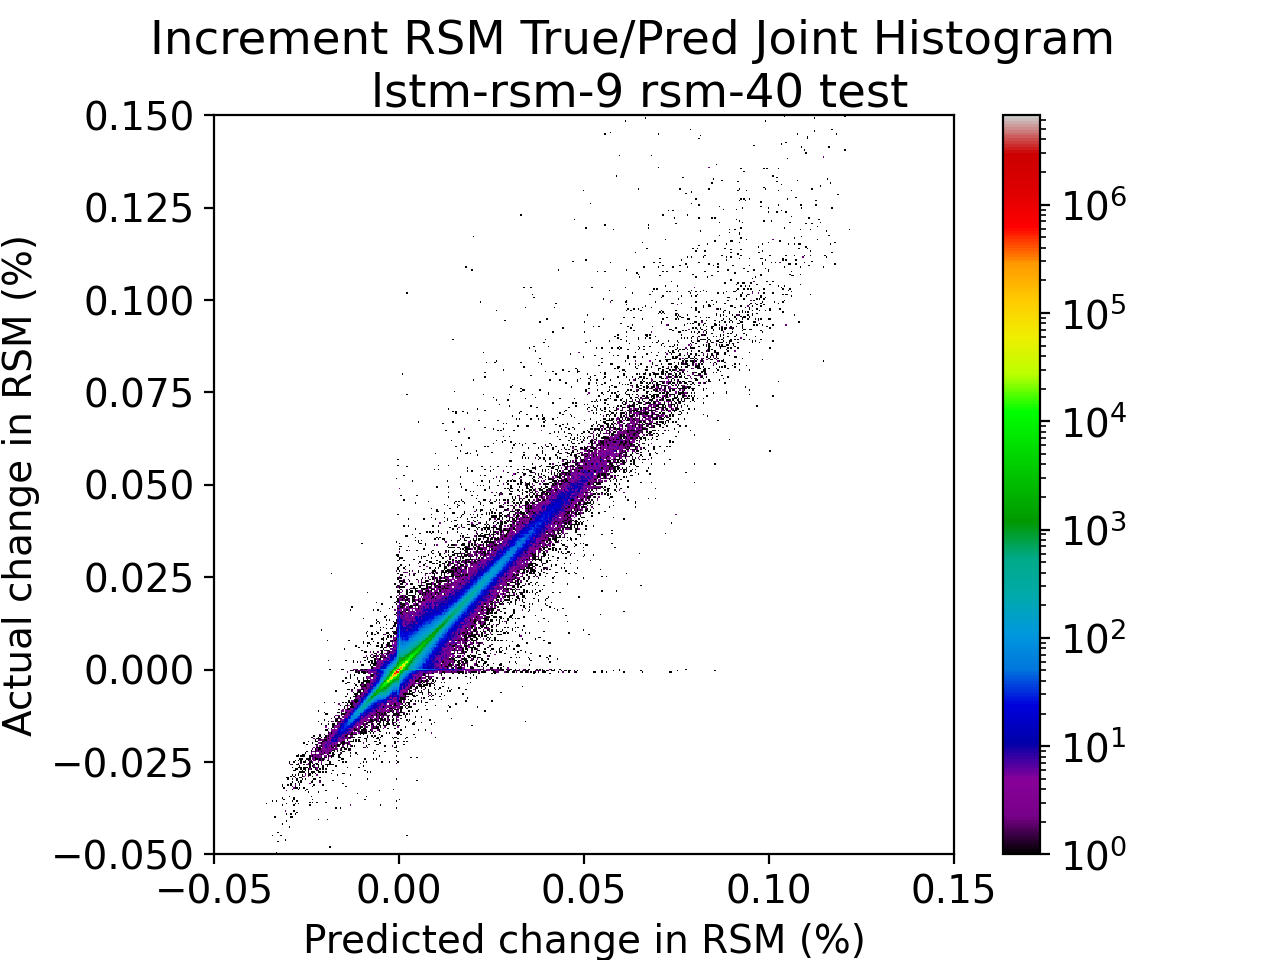
\includegraphics[width=.32\linewidth,draft=false]{figures/validation-curves/eval_test_lstm-rsm-9_rsm-40_hist-true-pred_na.png}
    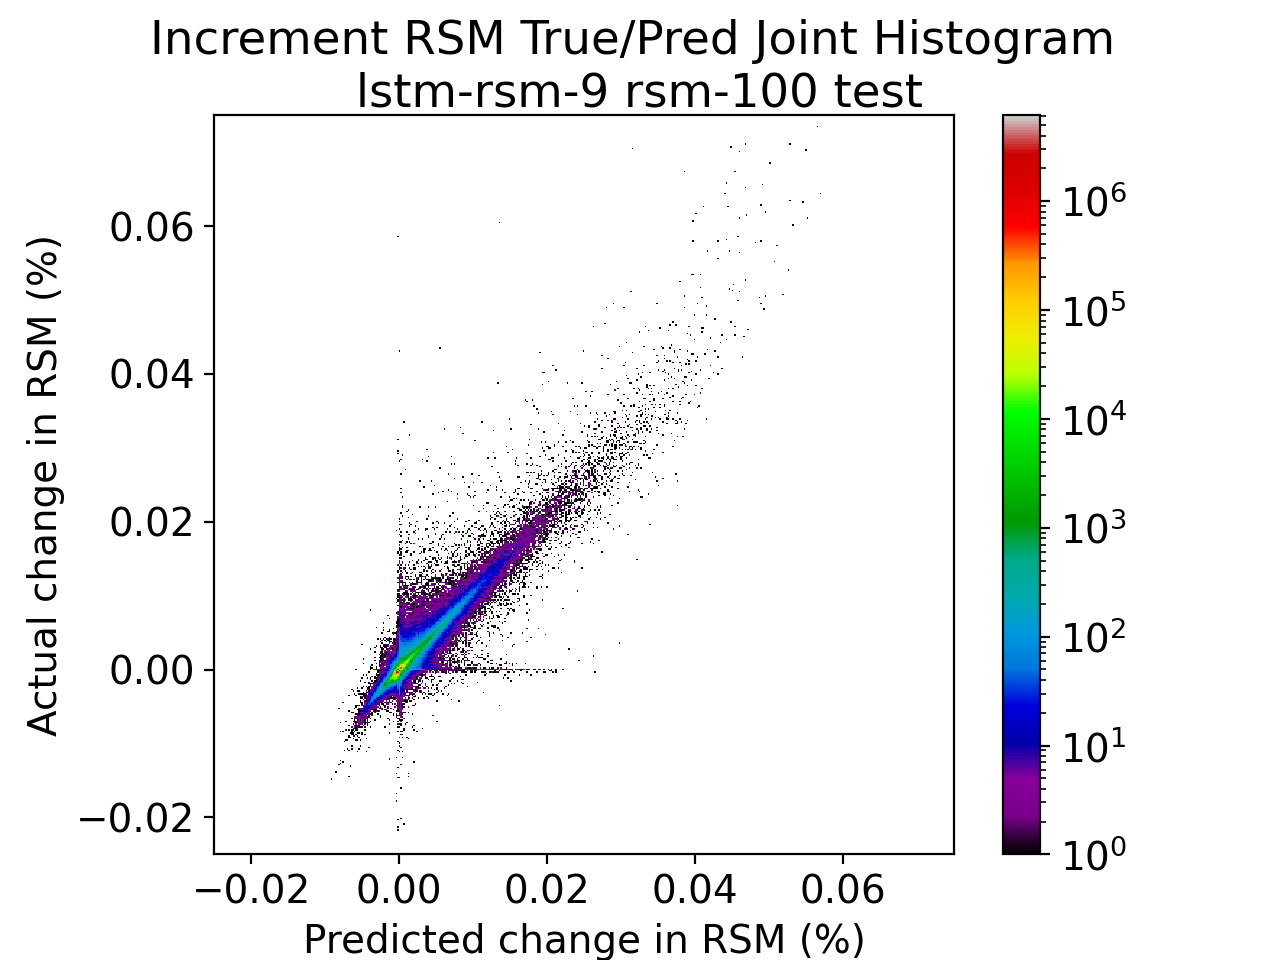
\includegraphics[width=.32\linewidth,draft=false]{figures/validation-curves/eval_test_lstm-rsm-9_rsm-100_hist-true-pred_na.png}

    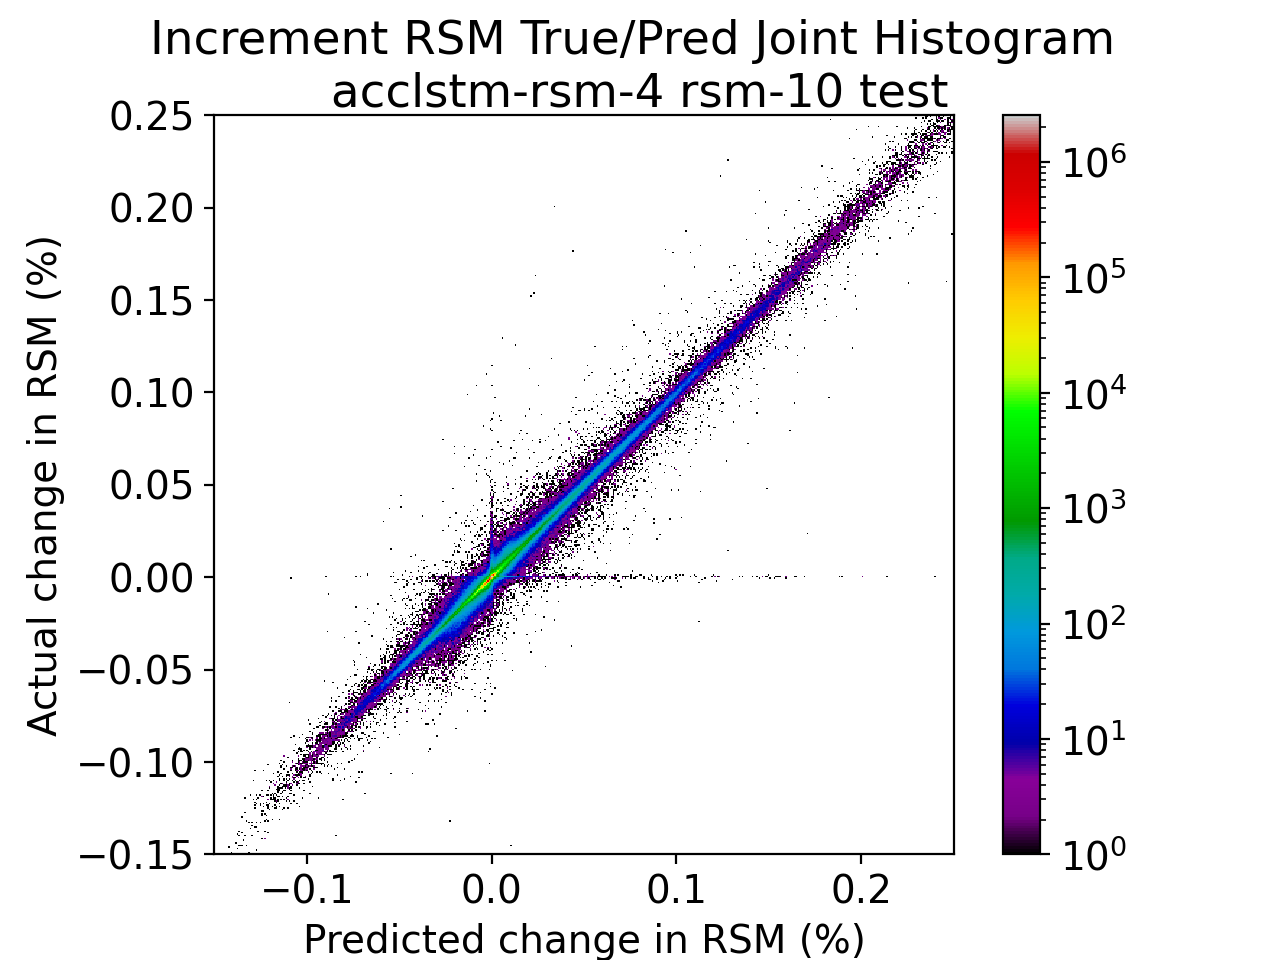
\includegraphics[width=.32\linewidth,draft=false]{figures/validation-curves/eval_test_acclstm-rsm-4_rsm-10_hist-true-pred_na.png}
    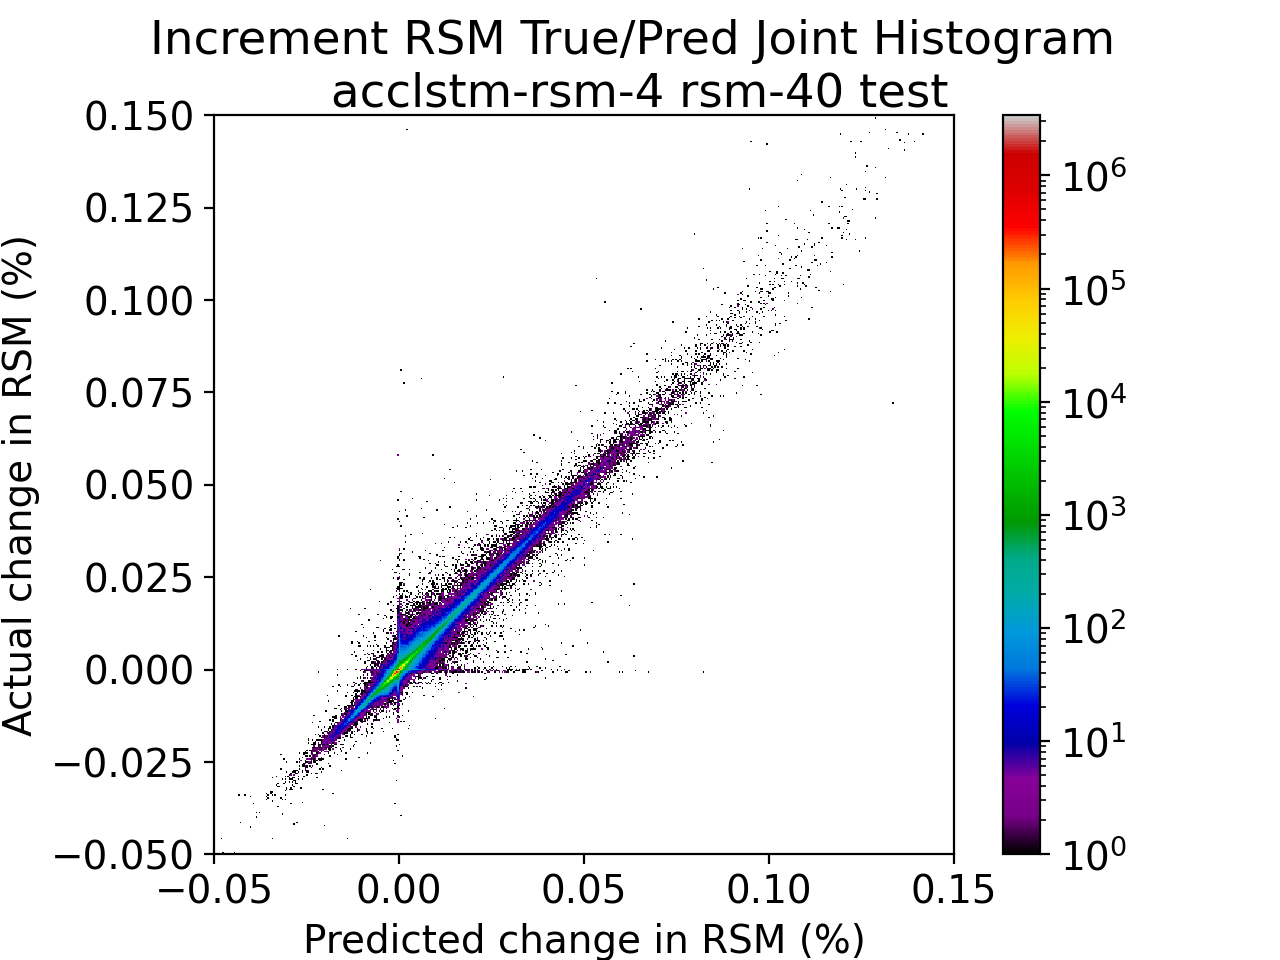
\includegraphics[width=.32\linewidth,draft=false]{figures/validation-curves/eval_test_acclstm-rsm-4_rsm-40_hist-true-pred_na.png}
    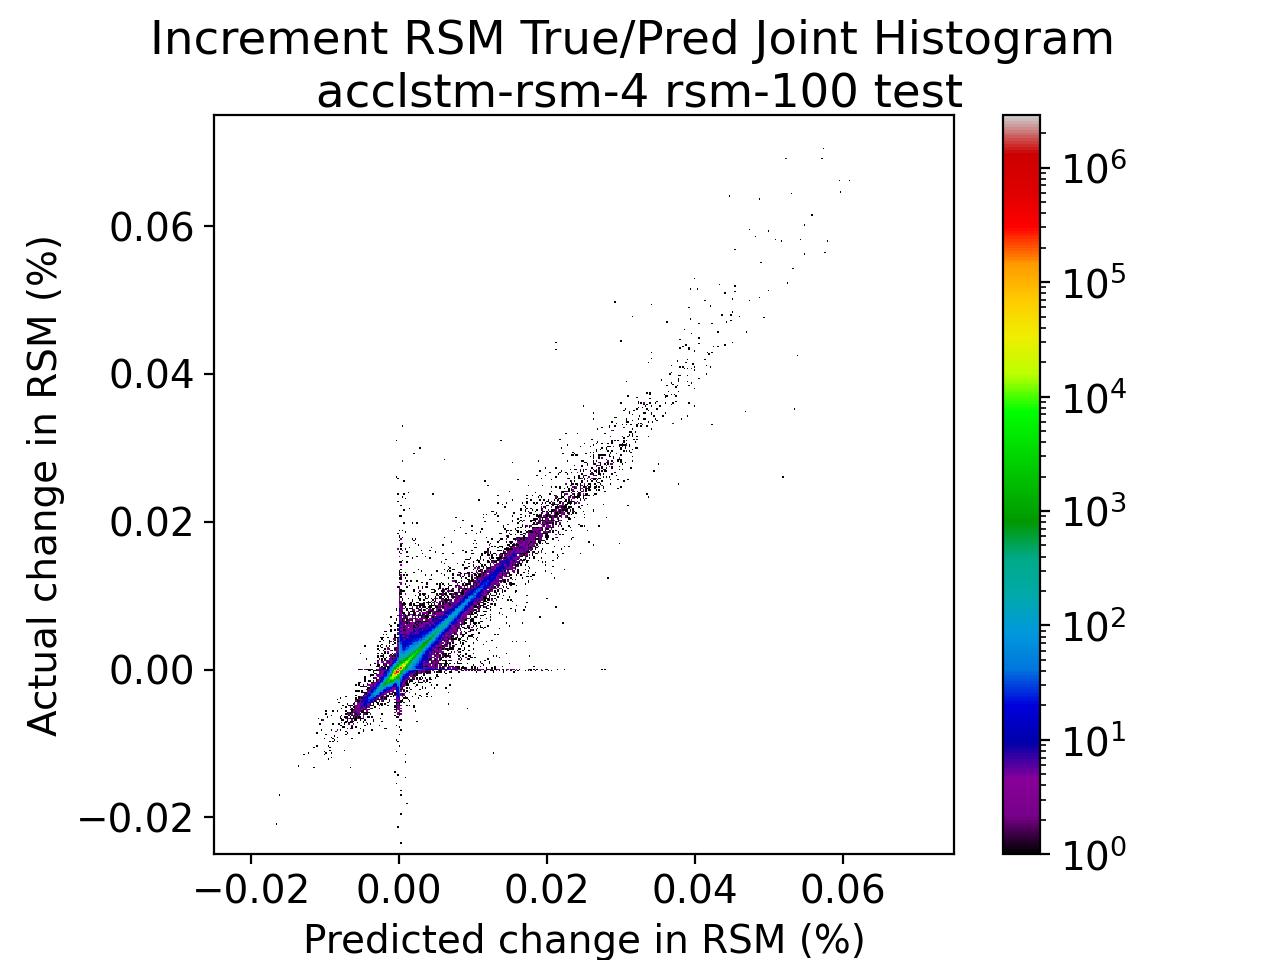
\includegraphics[width=.32\linewidth,draft=false]{figures/validation-curves/eval_test_acclstm-rsm-4_rsm-100_hist-true-pred_na.png}

    \caption{Heatmaps of true/predicted joint histograms for each of the top 3 soil layers, as predicted by the best models from each category.}
    \label{best-validation}
\end{figure}

\begin{figure}[hp!]
    \centering

    \includegraphics[width=.32\linewidth,draft=false]{figures/static-combos/eval_test_accfnn-rsm-8_rsm-10_static-combos_abs-err_state.png}
    \includegraphics[width=.32\linewidth,draft=false]{figures/static-combos/eval_test_accfnn-rsm-8_rsm-40_static-combos_abs-err_state.png}
    \includegraphics[width=.32\linewidth,draft=false]{figures/static-combos/eval_test_accfnn-rsm-8_rsm-100_static-combos_abs-err_state.png}

    \includegraphics[width=.32\linewidth,draft=false]{figures/static-combos/eval_test_lstm-20_rsm-10_static-combos_abs-err_state.png}
    \includegraphics[width=.32\linewidth,draft=false]{figures/static-combos/eval_test_lstm-20_rsm-40_static-combos_abs-err_state.png}
    \includegraphics[width=.32\linewidth,draft=false]{figures/static-combos/eval_test_lstm-20_rsm-100_static-combos_abs-err_state.png}

    \includegraphics[width=.32\linewidth,draft=false]{figures/static-combos/eval_test_lstm-rsm-9_rsm-10_static-combos_abs-err_state.png}
    \includegraphics[width=.32\linewidth,draft=false]{figures/static-combos/eval_test_lstm-rsm-9_rsm-40_static-combos_abs-err_state.png}
    \includegraphics[width=.32\linewidth,draft=false]{figures/static-combos/eval_test_lstm-rsm-9_rsm-100_static-combos_abs-err_state.png}

    \includegraphics[width=.32\linewidth,draft=false]{figures/static-combos/eval_test_acclstm-rsm-4_rsm-10_static-combos_abs-err_state.png}
    \includegraphics[width=.32\linewidth,draft=false]{figures/static-combos/eval_test_acclstm-rsm-4_rsm-40_static-combos_abs-err_state.png}
    \includegraphics[width=.32\linewidth,draft=false]{figures/static-combos/eval_test_acclstm-rsm-4_rsm-100_static-combos_abs-err_state.png}

    \caption{Absolute error of best models' state from each category with respect to static categorical parameter combinations.}
    \label{best-static-abserr}
\end{figure}

\begin{figure}[hp!]
    \centering

    \includegraphics[width=.32\linewidth,draft=false]{figures/static-combos/eval_test_accfnn-rsm-8_rsm-10_static-combos_bias_state.png}
    \includegraphics[width=.32\linewidth,draft=false]{figures/static-combos/eval_test_accfnn-rsm-8_rsm-40_static-combos_bias_state.png}
    \includegraphics[width=.32\linewidth,draft=false]{figures/static-combos/eval_test_accfnn-rsm-8_rsm-100_static-combos_bias_state.png}

    \includegraphics[width=.32\linewidth,draft=false]{figures/static-combos/eval_test_lstm-20_rsm-10_static-combos_bias_state.png}
    \includegraphics[width=.32\linewidth,draft=false]{figures/static-combos/eval_test_lstm-20_rsm-40_static-combos_bias_state.png}
    \includegraphics[width=.32\linewidth,draft=false]{figures/static-combos/eval_test_lstm-20_rsm-100_static-combos_bias_state.png}

    \includegraphics[width=.32\linewidth,draft=false]{figures/static-combos/eval_test_lstm-rsm-9_rsm-10_static-combos_bias_state.png}
    \includegraphics[width=.32\linewidth,draft=false]{figures/static-combos/eval_test_lstm-rsm-9_rsm-40_static-combos_bias_state.png}
    \includegraphics[width=.32\linewidth,draft=false]{figures/static-combos/eval_test_lstm-rsm-9_rsm-100_static-combos_bias_state.png}

    \includegraphics[width=.32\linewidth,draft=false]{figures/static-combos/eval_test_acclstm-rsm-4_rsm-10_static-combos_bias_state.png}
    \includegraphics[width=.32\linewidth,draft=false]{figures/static-combos/eval_test_acclstm-rsm-4_rsm-40_static-combos_bias_state.png}
    \includegraphics[width=.32\linewidth,draft=false]{figures/static-combos/eval_test_acclstm-rsm-4_rsm-100_static-combos_bias_state.png}

    \caption{Bias of best models' state from each category with respect to static categorical parameter combinations.}
    \label{best-static-bias}
\end{figure}

\section{Spatial, Temporal, and Situational Evaluation}

\section{Parameter Variations}

\section{Case Studies}

